\documentclass[11pt]{article}
\usepackage[margin=0.85in]{geometry}
\usepackage{amsmath,amssymb}
\usepackage{booktabs,array,graphicx}
\usepackage{microtype}
\usepackage{enumitem}
\usepackage{placeins}
\usepackage{hyperref}
\usepackage{xcolor}
\usepackage{multirow}
\usepackage{float}
\setlength{\parindent}{0pt}
\setlength{\parskip}{0.55\baselineskip}
\graphicspath{{figures/}}

\title{Compact ORCA Actuator Representations with MuJoCo-Constrained Temporal Refinement for Few-Shot Chinese Dance Gesture Recognition}
\author{Jiating Li\\\small \textbf{[TODO: affiliation]}\\\small \textbf{[TODO: institutional email and corresponding-author marker]}}
\date{}

\begin{document}
\maketitle

\begin{abstract}
Monocular hand landmarks provide an accessible input for gesture recognition, but their high dimensionality and temporal instability are problematic when training data are limited. This paper presents a structured representation pipeline for Chinese dance hand gestures. MediaPipe landmarks are first mapped frame by frame to a 17-dimensional actuator state of an ORCA articulated hand. The state is then refined causally using MuJoCo forward kinematics, robust observation fitting, actuator bounds, and first- and second-order temporal regularization. A development-only selection procedure further freezes a seven-actuator semantic subset, Compact Refined-7, before final-test evaluation. Experiments use 571 sequences from six gesture classes. Within actuator space, temporal refinement reduces mean velocity from 0.4590 to 0.2470 and mean acceleration from 0.7100 to 0.2703, corresponding to reductions of 46.2\% and 61.9\%. Under controlled landmark corruption, refinement reduces the overall actuator deviation from 0.0292 to 0.0182, a 37.6\% reduction relative to Actuator Projection-17. On the frozen 115-sequence final test, Compact Refined-7 uses 112 sequence features and outperforms the published-definition JointAngle-11 baseline with SVM and KNN after Holm correction, while the RandomForest and MLP differences are not significant. These findings support a bounded claim: ORCA embodiment provides a compact semantic state, MuJoCo-constrained temporal refinement improves its stability and perturbation robustness, and a frozen semantic subset can preserve or improve recognition performance without claiming ground-truth 3D pose recovery.
\end{abstract}

\textbf{Keywords:} hand gesture recognition; MediaPipe; MuJoCo; actuator representation; temporal refinement; few-shot learning; Chinese dance

\section{Introduction}

Hand gestures in Chinese dance are defined by coordinated finger flexion, thumb articulation, and palm configuration. Vision-based capture avoids gloves and markers, but practical monocular trackers can produce jitter, transient spikes, and unstable joint configurations under oblique viewpoints, rapid movement, and self-occlusion. These errors matter in few-shot recognition because subtle classes must be separated using only a small number of labeled sequences.

MediaPipe Hands provides an efficient landmark detector and lightweight tracking pipeline~\cite{zhang2020mediapipehands}. Existing gesture-recognition systems commonly treat estimated landmarks as ready-to-use features and focus on the temporal classifier. This leaves two representation problems unresolved. First, 21 three-dimensional landmarks form a 63-dimensional coordinate vector containing nuisance variation. Second, coordinate-space smoothing can reduce high-frequency variation without enforcing compatibility with an articulated hand model.

This work asks whether an embodied actuator space can provide a more compact and stable intermediate representation. The pipeline maps landmarks to the 17 actuators of an ORCA hand, refines the actuator trajectory through MuJoCo forward kinematics and causal temporal regularization, and evaluates the representation with lightweight classifiers. Classification is used to evaluate representation utility; it is not the denoising mechanism.

The study addresses four research questions:
\begin{description}[leftmargin=0.75in,style=nextline]
\item[RQ1] How does the 17-dimensional actuator projection reorganize MediaPipe landmarks into a bounded semantic state, and how does it compare with other structured representations under dimension-controlled evaluation?
\item[RQ2] Does MuJoCo-constrained causal refinement reduce actuator-space temporal variation and sensitivity to controlled landmark corruption?
\item[RQ3] Can a development-selected semantic actuator subset retain useful information with fewer dimensions?
\item[RQ4] On a frozen final test, how does Compact Refined-7 compare with a conventional 11-dimensional 3D joint-angle representation across classifiers?
\end{description}

The contributions are:
\begin{enumerate}[leftmargin=*]
\item An embodiment-aware mapping from MediaPipe landmarks to a 17-dimensional ORCA actuator state, providing an interpretable alternative to raw coordinates and generic dimensionality reduction.
\item A causal MuJoCo-constrained objective combining robust landmark fitting, palm orientation, actuator priors, hard bounds, and temporal regularization. Its main demonstrated benefit is reduced temporal variation and reduced actuator sensitivity under controlled input corruption.
\item A development-only selection procedure that freezes seven semantically distributed flexion actuators before final evaluation. Compact Refined-7 reduces encoded dimensionality by 58.8\% relative to Refined ORCA-17 and by 36.4\% relative to JointAngle-11.
\item A dimension- and classifier-controlled evaluation using a frozen 456/115 development/final split, common few-shot splits, confidence intervals, paired Wilcoxon tests, Holm correction, and effect sizes.
\end{enumerate}

We do not treat MuJoCo output as ground-truth human 3D pose, call controlled corruption physical pose recovery, or claim that refinement improves every classifier.

\begin{figure}[t]
\centering
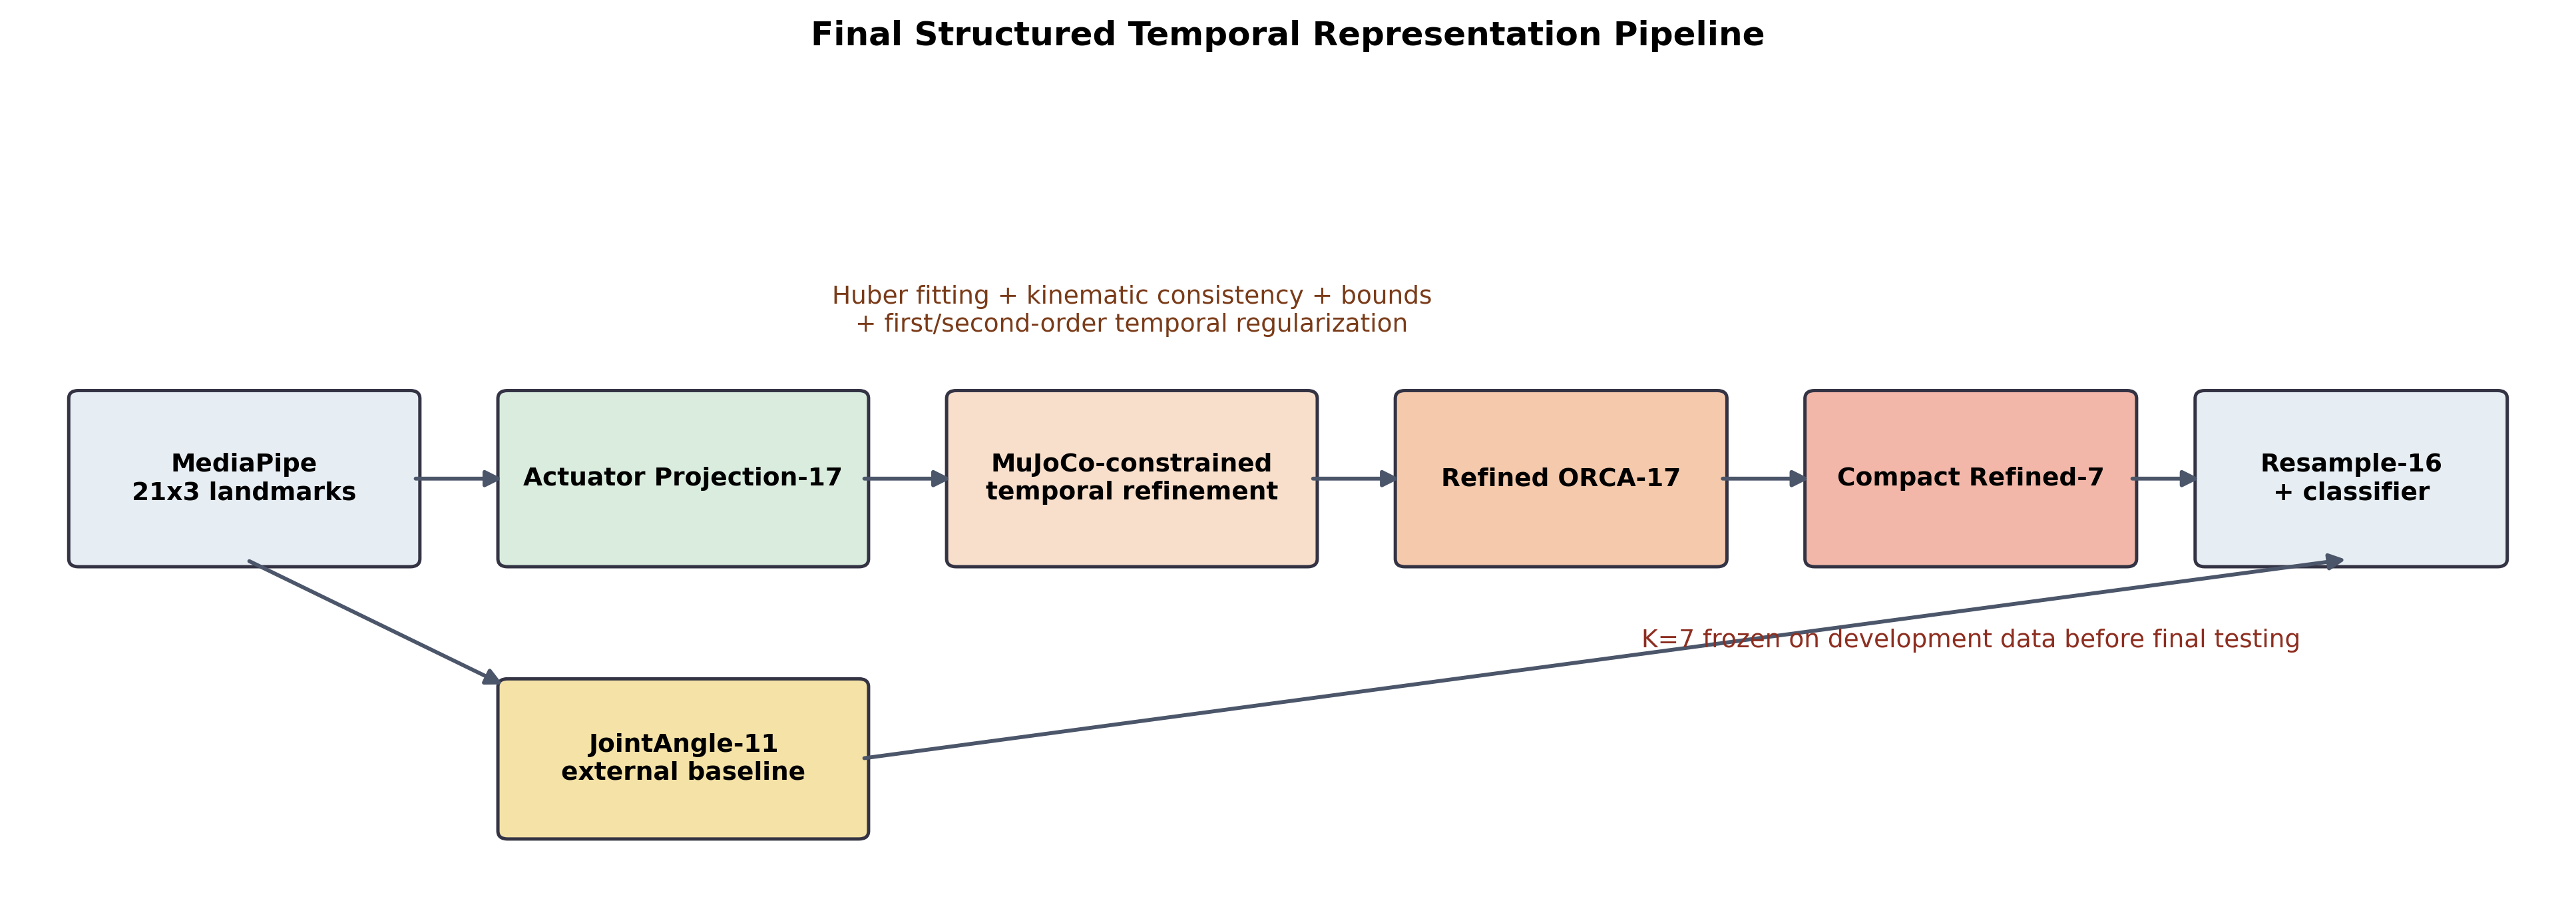
\includegraphics[width=\linewidth]{figure_01_final_pipeline.png}
\caption{Frozen scientific pipeline. Actuator Projection-17 supplies a structured initialization, MuJoCo optimization produces Refined ORCA-17, and Compact Refined-7 provides a development-selected semantic readout.}
\label{fig:pipeline}
\end{figure}

\section{Related Work}

\subsection{Vision-based hand landmarks}
MediaPipe Hands combines palm detection with landmark estimation for real-time use~\cite{zhang2020mediapipehands}. Monocular hand pose remains ambiguous under self-occlusion and viewpoint changes~\cite{zimmermann2017learning,boukhayma2019handwild}. Gesture-recognition studies therefore explore RGB, skeleton, and landmark representations~\cite{caputo2021shrec,kopuklu2020drivermhg,kapitanov2022hagrid}.

\subsection{Structured hand representations}
Joint angles describe local geometry, while articulated models restrict motion to meaningful degrees of freedom. MANO illustrates the value of compact hand parameterization~\cite{romero2017embodied}. The ORCA actuator state used here is not asserted to be anatomically identical to a human hand; it is an interpretable, bounded latent space.

\subsection{Filtering and constrained refinement}
Savitzky--Golay filtering~\cite{savitzky1964smoothing}, the One Euro filter~\cite{casiez2012oneeuro}, and Kalman filtering~\cite{kalman1960new} suppress temporal noise directly in coordinate space. They do not impose ORCA kinematics. MuJoCo provides a forward model for articulated systems~\cite{todorov2012mujoco}. Our use is kinematic and optimization based, not a claim of force, torque, contact, or human dynamics recovery.

\subsection{Few-shot evaluation}
Few-shot learning emphasizes representation quality when labels are scarce~\cite{vinyals2016matching,snell2017prototypical}. We intentionally use lightweight downstream classifiers so that representation differences remain visible.

\section{Method}

\subsection{Overview and notation}
Let $\mathbf{Y}_t\in\mathbb{R}^{21\times3}$ denote MediaPipe landmarks and $\mathbf{q}_t\in\mathbb{R}^{17}$ the ORCA actuator state. Figure~\ref{fig:pipeline} separates three roles: structured frame-wise initialization, causal temporal refinement, and compact readout.

\subsection{Actuator Projection-17}
The projection is
\begin{equation}
\tilde{\mathbf q}_t=g(\mathbf Y_t),\qquad \tilde{\mathbf q}_t\in\mathbb R^{17}.
\end{equation}
The deterministic map $g$ converts wrist-normalized landmark vectors into palm orientation, finger abduction, finger flexion, and thumb articulation features, then maps each feature to the corresponding ORCA actuator range. The legacy feature key is \texttt{corrected}; the manuscript consistently calls it \emph{Actuator Projection-17} because it is a deterministic projection rather than an optimization output.

For landmarks $\mathbf a,\mathbf b,\mathbf c$, the implementation computes the included angle
\begin{equation}
\theta(\mathbf a,\mathbf b,\mathbf c)=\cos^{-1}\!\left(\frac{(\mathbf a-\mathbf b)^\top(\mathbf c-\mathbf b)}{\|\mathbf a-\mathbf b\|_2\|\mathbf c-\mathbf b\|_2}\right),
\end{equation}
and maps finger flexion by $f(\theta)=\operatorname{clip}((175-\theta_{\rm deg})/95,0,1)$. Signed spread about the palm normal is
\begin{equation}
\phi(\mathbf v_1,\mathbf v_2,\mathbf n)=\operatorname{atan2}((\mathbf v_1\times\mathbf v_2)^\top\mathbf n,\mathbf v_1^\top\mathbf v_2),
\end{equation}
followed by $\operatorname{clip}(\phi_{\rm deg}/25,-1,1)$. The palm basis uses wrist-to-middle-MCP as the forward vector, pinky-MCP-to-index-MCP as the across vector, and their normalized forward--across cross product as the normal. Wrist flexion is obtained from $\operatorname{atan2}(-v_z,|v_y|)$ and clipped after division by $55^\circ$. Thumb opening combines planar opening and normalized thumb-tip--index-MCP distance with weights 0.7 and 0.3. Unit features are mapped linearly to actuator limits; signed features are mapped around the range midpoint or neutral MuJoCo state. Table~\ref{tab:actuators} provides the exact box limits in radians.

\begin{figure}[t]
\centering
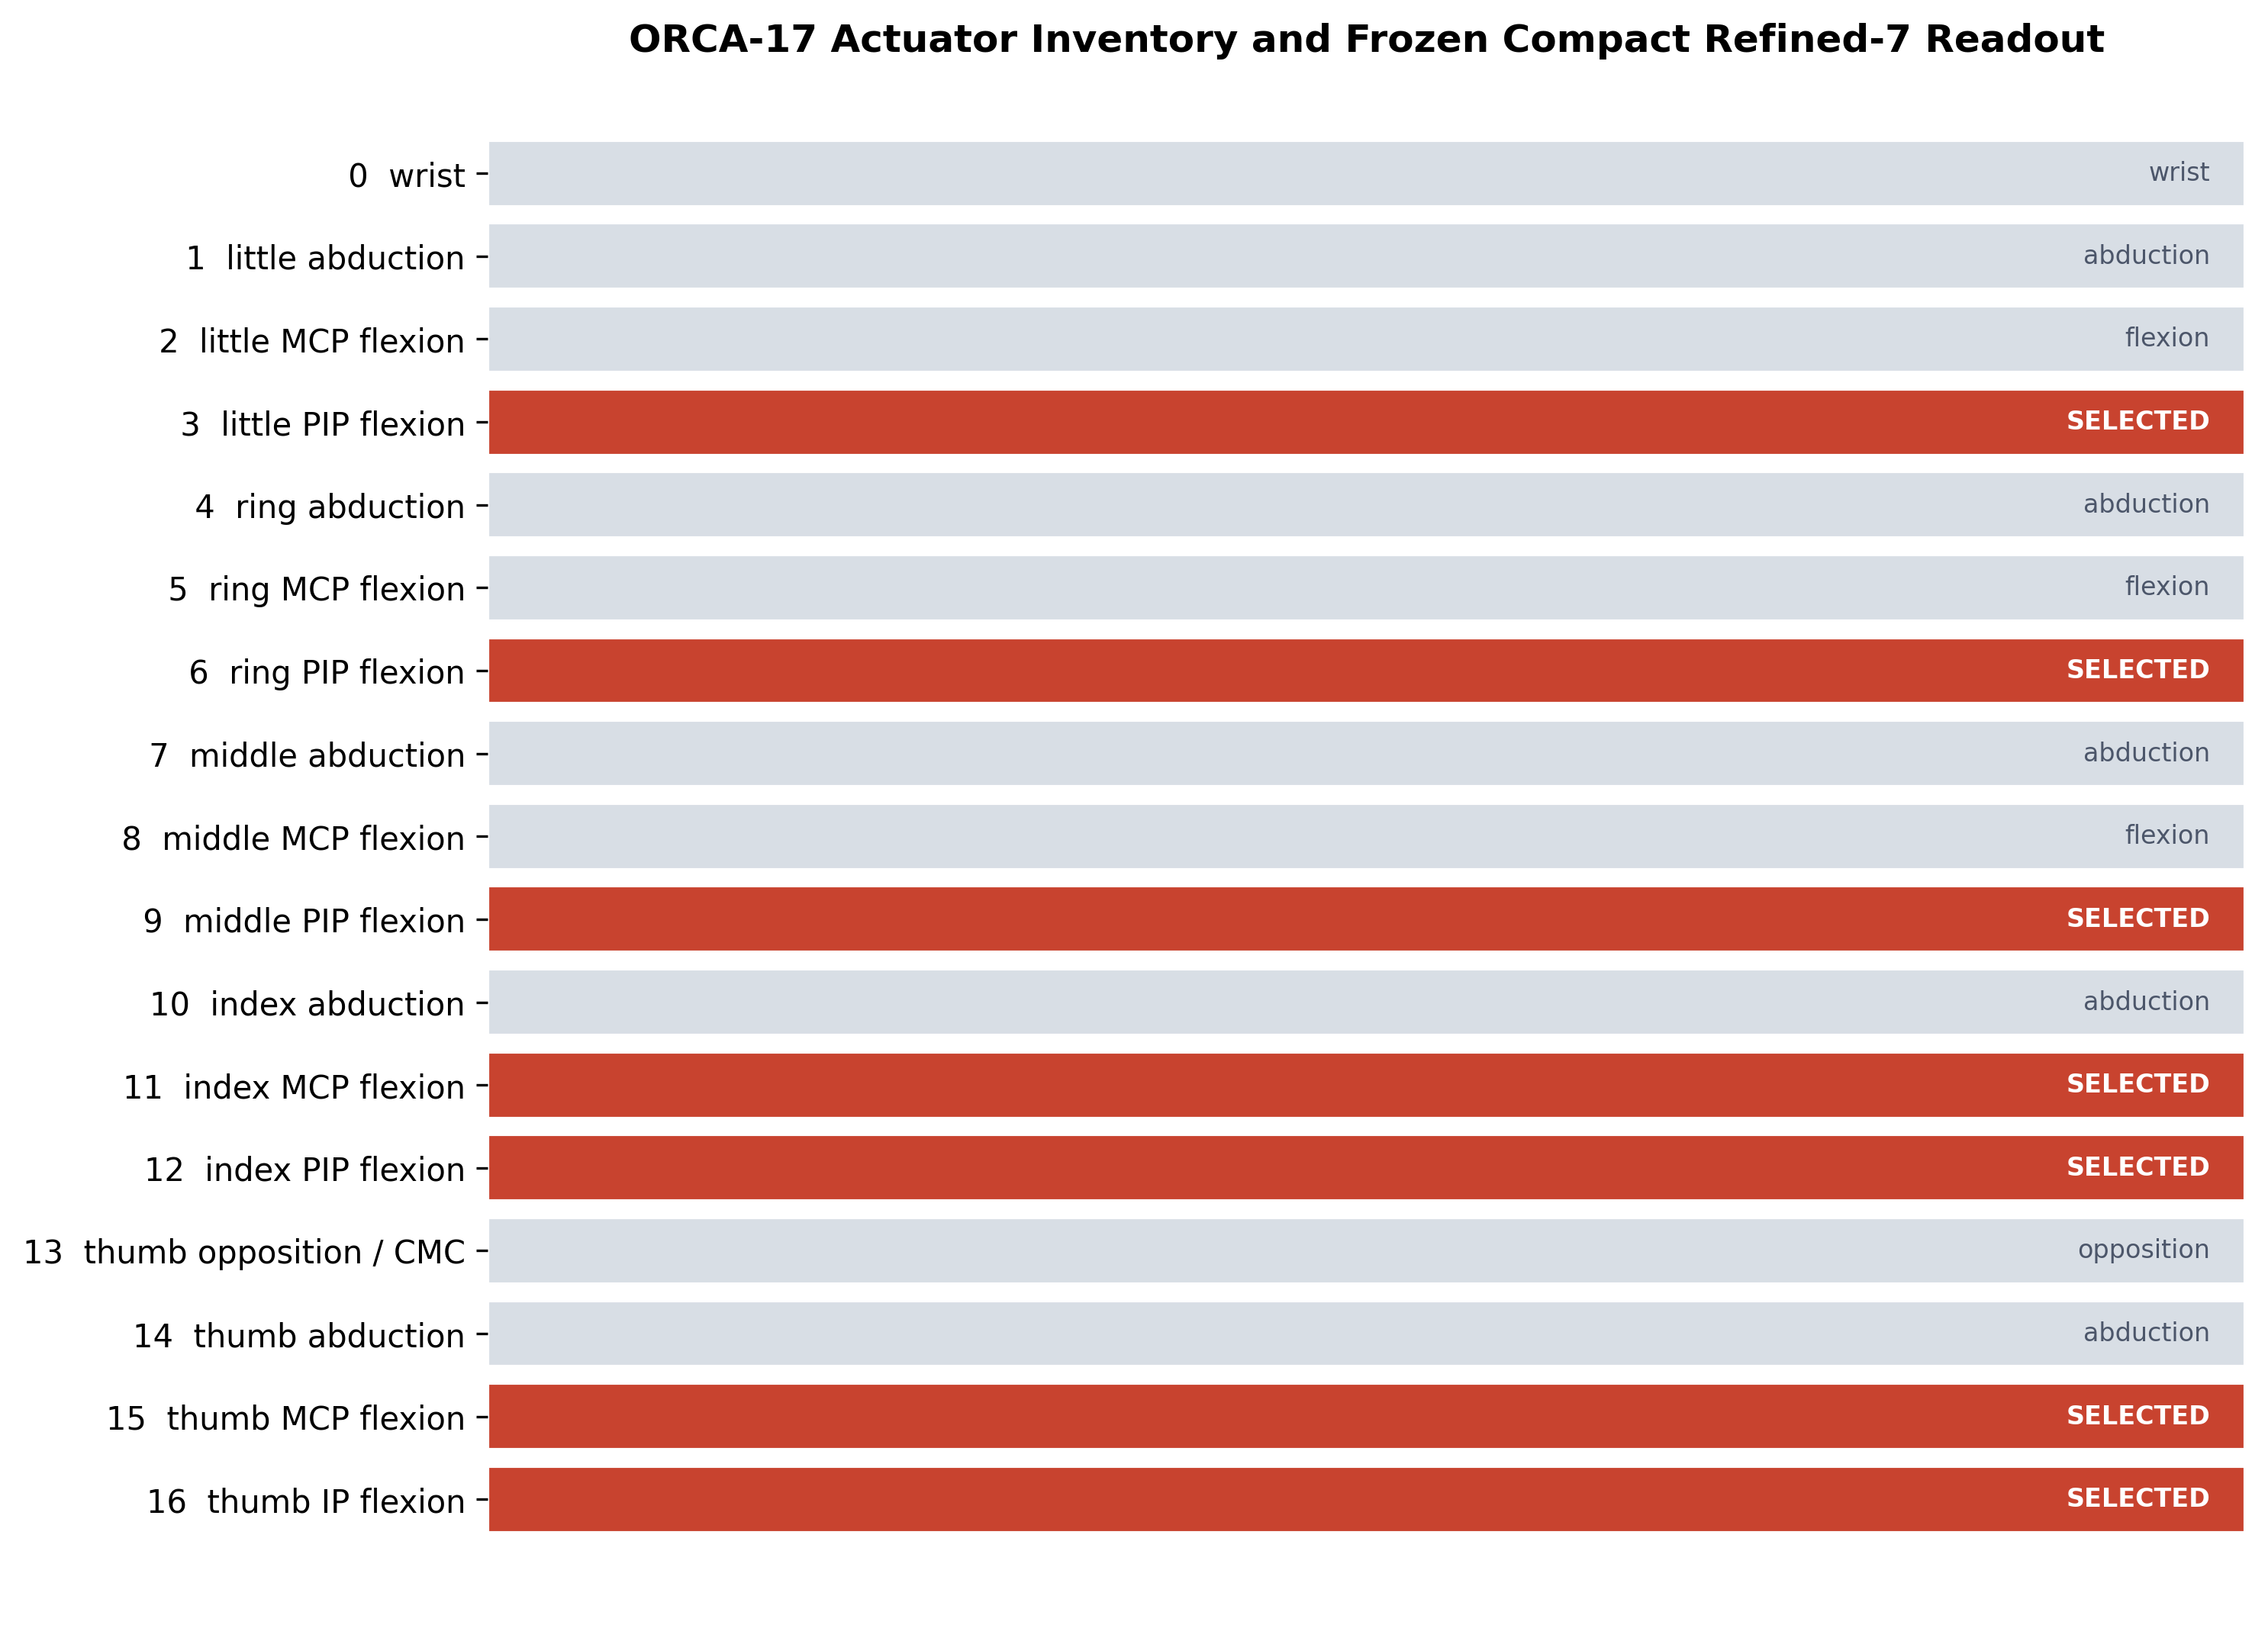
\includegraphics[width=\linewidth]{figure_02_orca_actuator_structure.png}
\caption{The 17 ORCA actuator channels and the seven frozen Compact ORCA channels.}
\label{fig:actuators}
\end{figure}

\begin{table}[t]
\centering
\caption{ORCA actuator inventory.}
\label{tab:actuators}
\scriptsize
\resizebox{\linewidth}{!}{\begin{tabular}{rllllrrc}
\toprule
Index & Actuator & Role & Group & Type & Low (rad) & High (rad) & Compact7 \\
\midrule
0 & right\_wrist\_actuator & wrist & wrist & wrist & -1.1345 & 0.6109 & no \\
1 & right\_p-abd\_actuator & little abduction & little & abduction & -0.5236 & 0.5236 & no \\
2 & right\_p-mcp\_actuator & little MCP flexion & little & flexion & -0.4363 & 1.7453 & no \\
3 & right\_p-pip\_actuator & little PIP flexion & little & flexion & -0.2618 & 1.8675 & yes \\
4 & right\_r-abd\_actuator & ring abduction & ring & abduction & -0.4712 & 0.4712 & no \\
5 & right\_r-mcp\_actuator & ring MCP flexion & ring & flexion & -0.4363 & 1.7453 & no \\
6 & right\_r-pip\_actuator & ring PIP flexion & ring & flexion & -0.2618 & 1.8675 & yes \\
7 & right\_m-abd\_actuator & middle abduction & middle & abduction & -0.4712 & 0.4712 & no \\
8 & right\_m-mcp\_actuator & middle MCP flexion & middle & flexion & -0.4363 & 1.7453 & no \\
9 & right\_m-pip\_actuator & middle PIP flexion & middle & flexion & -0.2618 & 1.8675 & yes \\
10 & right\_i-abd\_actuator & index abduction & index & abduction & -0.4363 & 0.5236 & no \\
11 & right\_i-mcp\_actuator & index MCP flexion & index & flexion & -0.4363 & 1.7453 & yes \\
12 & right\_i-pip\_actuator & index PIP flexion & index & flexion & -0.2618 & 1.8675 & yes \\
13 & right\_t-cmc\_actuator & thumb opposition / CMC & thumb & opposition & -0.7854 & 0.5760 & no \\
14 & right\_t-abd\_actuator & thumb abduction & thumb & abduction & -0.3142 & 0.9599 & no \\
15 & right\_t-mcp\_actuator & thumb MCP flexion & thumb & flexion & -0.4363 & 1.7453 & yes \\
16 & right\_t-pip\_actuator & thumb IP flexion & thumb & flexion & -0.2618 & 1.8675 & yes \\
\bottomrule
\end{tabular}
}
\end{table}

\subsection{MuJoCo-constrained causal temporal refinement}
Let $h(\mathbf q)$ be the MuJoCo forward-kinematic mapping and $\mathcal Q$ the actuator box. The refined state is
\begin{align}
\mathbf q_t^*=\arg\min_{\mathbf q_t\in\mathcal Q}\;&
\lambda_l\mathcal L_{\mathrm{huber}}+
\lambda_n\mathcal L_{\mathrm{normal}}+
\lambda_p\mathcal L_{\mathrm{prior}}+
\lambda_s\mathcal L_{\mathrm{temporal}} \nonumber\\
&+\lambda_a\mathcal L_{\mathrm{acceleration}}+
\lambda_d\mathcal L_{\mathrm{default}}+
\lambda_b\mathcal L_{\mathrm{boundary}}.
\label{eq:objective}
\end{align}
Hard box limits are enforced by L-BFGS-B.

The fixed objective weights are $\lambda_l=1.00$, $\lambda_n=0.20$, $\lambda_p=0.30$, $\lambda_s=0.10$, $\lambda_a=0.15$, $\lambda_d=0.15$, and $\lambda_b=0.05$, with Huber threshold $\delta=0.08$. SciPy L-BFGS-B is initialized from the clipped Actuator Projection-17 state, permits at most 120 iterations per frame, and otherwise uses SciPy's default stopping tolerances. No objective weight is tuned per sequence or corruption condition.

\begin{table}[t]
\centering
\caption{Frozen temporal-refinement parameters.}
\label{tab:optimizerparams}
\small
\begin{tabular}{lll}
\toprule
Parameter & Symbol & Value \\
\midrule
landmark weight & lambda\_l & 1.00 \\
palm-normal weight & lambda\_n & 0.20 \\
projection-prior weight & lambda\_p & 0.30 \\
first-order temporal weight & lambda\_s & 0.10 \\
acceleration weight & lambda\_a & 0.15 \\
neutral-pose weight & lambda\_d & 0.15 \\
soft-boundary weight & lambda\_b & 0.05 \\
Huber threshold & delta & 0.08 \\
optimizer & -- & SciPy L-BFGS-B \\
maximum iterations per frame & -- & 120 \\
initialization & -- & clipped actuator projection \\
other stopping tolerances & -- & SciPy defaults \\
\bottomrule
\end{tabular}

\end{table}

Eight correspondences are used: wrist, thumb tip, index MCP/tip, middle MCP/tip, and little MCP/tip. For $r_{t,i,k}=h_i(\mathbf q_t)_k-Y_{t,i,k}$,
\begin{equation}
\mathcal L_{\mathrm{huber}}=\sum_{i\in\mathcal C}\sum_{k=1}^{3}\rho_\delta(r_{t,i,k}),
\end{equation}
where the component-wise Huber penalty~\cite{huber1964robust} is
\begin{equation}
\rho_\delta(r)=
\begin{cases}
\frac{1}{2}r^2,& |r|\leq\delta,\\
\delta\left(|r|-\frac{1}{2}\delta\right),& |r|>\delta.
\end{cases}
\end{equation}
The remaining main terms are
\begin{align}
\mathcal L_{\mathrm{normal}}&=\|\mathbf n_{\mathrm{orca}}(\mathbf q_t)-\mathbf n_{\mathrm{mp}}(\mathbf Y_t)\|_2^2,\\
\mathcal L_{\mathrm{prior}}&=\|\mathbf q_t-\tilde{\mathbf q}_t\|_2^2,\\
\mathcal L_{\mathrm{temporal}}&=\|\mathbf q_t-\mathbf q_{t-1}^*\|_2^2,\\
\mathcal L_{\mathrm{acceleration}}&=\|\mathbf q_t-2\mathbf q_{t-1}^*+\mathbf q_{t-2}^*\|_2^2.
\end{align}
Both palm normals use the same cross-product convention; a MuJoCo-generated regression test verifies a dot product close to $+1$.

Let $\mathbf q^0$ be the neutral state:
\begin{equation}
\mathcal L_{\mathrm{default}}=\|\mathbf q_t-\mathbf q^0\|_2^2.
\end{equation}
For limits $q_j^{\min},q_j^{\max}$, define
\begin{equation}
u_{t,j}=\frac{q_{t,j}-q_j^{\min}}{\max(q_j^{\max}-q_j^{\min},10^{-6})}.
\end{equation}
The soft outer-range penalty is
\begin{equation}
\mathcal L_{\mathrm{boundary}}=\sum_j\left[\max(0,0.1-u_{t,j})^2+\max(0,u_{t,j}-0.9)^2\right].
\end{equation}
It complements, rather than replaces, hard bounds. At the first frame both temporal terms are zero; at the second only the first-order term is active. History is reset at every sequence boundary.

Before fitting, both point sets are translated to the wrist and divided by
\begin{equation}
s_t=\max\left(\|\mathbf Y_{t,\mathrm{indexMCP}}-\mathbf Y_{t,\mathrm{pinkyMCP}}\|_2,
\|\mathbf Y_{t,\mathrm{middleMCP}}-\mathbf Y_{t,\mathrm{wrist}}\|_2,10^{-6}\right).
\end{equation}
The acquisition uses right-hand observations and the right-hand ORCA model; it is not a general left/right canonicalization procedure. Reconstructed model points are $\mathbf Y_t^*=h(\mathbf q_t^*)$. They use the legacy feature key \texttt{optimized\_full} and are called \emph{Reconstructed ORCA Landmarks} in the manuscript.

\subsection{Frozen Compact Refined-7}
Actuator selection uses development data only. Candidate channels are scored by
\begin{equation}
U_j=D_j-0.25W_j-0.20I_j-0.15R_j-0.15S_j,
\end{equation}
Here $D_j$ is the min--max-scaled $\log(1+F_j)$ obtained from a sequence-level ANOVA statistic; $W_j$ is min--max-scaled within-class variance; $I_j$ is min--max-scaled first- plus second-difference RMS; $R_j$ is the maximum absolute Pearson correlation with another channel; and $S_j$ penalizes reduced discriminative utility or increased instability after refinement. The components are calculated after development-partition standardization. Candidate values $K\in\{5,7,9,11,13\}$ are compared using $0.3\,\mathrm{Accuracy}+0.7\,\mathrm{MacroF1}$ averaged over four classifiers. The smallest candidate within one standard error of the best mean is selected, subject to one channel from each thumb/finger group. The error bars in Figure~\ref{fig:development} are 95\% confidence intervals, $1.96s/\sqrt{20}$, rather than standard deviations. This procedure selected $K=7$ before the final test; the frozen indices are $[3,6,9,11,12,15,16]$.

\begin{table}[t]
\centering
\caption{Frozen Compact Refined-7 channels.}
\label{tab:compact7}
\scriptsize
\begin{tabular}{rll}
\toprule
Index & Actuator & Role \\
\midrule
3 & right\_p-pip\_actuator & little PIP flexion \\
6 & right\_r-pip\_actuator & ring PIP flexion \\
9 & right\_m-pip\_actuator & middle PIP flexion \\
11 & right\_i-mcp\_actuator & index MCP flexion \\
12 & right\_i-pip\_actuator & index PIP flexion \\
15 & right\_t-mcp\_actuator & thumb MCP flexion \\
16 & right\_t-pip\_actuator & thumb IP flexion \\
\bottomrule
\end{tabular}

\end{table}

\subsection{Sequence encoding and baselines}
For $\mathbf X\in\mathbb R^{T\times d}$, linear interpolation resamples each feature trajectory to 16 normalized time positions, yielding $\mathrm{Resample16}(\mathbf X)\in\mathbb R^{16d}$. This is the primary order-preserving encoder. The earlier mean/std/max/delta summary remains an order-light supporting baseline only.

JointAngle-11 computes conventional 3D landmark-vector angles using a published geometric definition. It is an external representation baseline, not a full reproduction of the source paper's dataset and system. PCA is fitted on training data only~\cite{jolliffe2002pca}.

\begin{table}[t]
\centering
\caption{Representation dimensions and Resample16 encoded sizes.}
\label{tab:dimensions}
\small
\begin{tabular}{lrrl}
\toprule
Representation & Frame dim. & Resample16 & Role \\
\midrule
Raw landmarks & 63 & 1008 & Cartesian observations \\
JointAngle-11 & 11 & 176 & 3D included angles \\
Actuator Projection-17 & 17 & 272 & Frame-wise ORCA state \\
Refined ORCA-17 & 17 & 272 & Refined ORCA state \\
Projection/Refined Flex-11 & 11 & 176 & Predefined semantic subset \\
Compact Projection/Refined-7 & 7 & 112 & Development-selected frozen subset \\
Projection/Refined PCA-11 & 11 & 176 & Training-only statistical control \\
\bottomrule
\end{tabular}

\end{table}

\FloatBarrier
\section{Experimental Protocol}

\subsection{Dataset and frozen split}
The dataset contains 571 sequences and 26,260 frames from six Chinese dance gesture classes: deer horn, flower pinch, orchid finger, orchid palm, prayer beads, and three-finger bent. A frozen split assigns 456 sequences to development and 115 to final testing. Selection uses development data only; the final partition is used once after freezing Compact Refined-7. The dataset does not yet establish subject-independent generalization.

Before submission, the following acquisition records must be inserted from the study log rather than inferred from the CSV: \textbf{[TODO: participant count]}, \textbf{[TODO: sessions per participant]}, \textbf{[TODO: per-class distribution]}, \textbf{[TODO: camera/device]}, \textbf{[TODO: resolution and frame rate]}, \textbf{[TODO: distance, lighting, and background protocol]}, and \textbf{[TODO: handling of failed MediaPipe frames]}.

\subsection{Few-shot evaluation}
The primary evaluation uses three labeled training sequences per class and 20 common repeated splits. Sampling occurs at sequence level, never at frame level, and the same sequence identifiers are used for all representations within a repeat. Standardization and PCA are fitted only on training samples. Frozen settings are RBF-SVM ($C=5$, $\gamma=\texttt{scale}$), distance-weighted KNN ($k=3$), RandomForest (200 trees, unrestricted depth), and MLP (hidden layers 128 and 64, $\alpha=10^{-4}$, initial learning rate $10^{-3}$, maximum 1200 iterations). Every estimator is wrapped in a training-only StandardScaler pipeline.

We report accuracy, macro-F1, and Cohen's kappa with dispersion and 95\% confidence intervals. Paired comparisons use repeat-wise Wilcoxon signed-rank tests and Cohen's $d_z$. Holm correction is applied separately for each classifier--metric pair over six predefined representation comparisons. Because all repeats share the same frozen 115-sequence final partition, these intervals quantify variation from few-shot training-sequence selection rather than uncertainty for unseen participants or datasets.

\begin{table}[t]
\centering
\caption{Frozen downstream-classifier settings.}
\label{tab:classifierparams}
\small
\begin{tabular}{ll}
\toprule
Classifier & Frozen setting \\
\midrule
SVM & RBF kernel; C=5; gamma=scale \\
KNN & k=3; distance weighting \\
RandomForest & 200 trees; unrestricted depth \\
MLP & hidden=(128,64); alpha=1e-4; lr=1e-3; max\_iter=1200 \\
\bottomrule
\end{tabular}

\end{table}

\subsection{Stability, perturbation, ablation, and runtime}
Actuator velocity and acceleration are compared only within the common 17-dimensional actuator space. Controlled corruption is applied in normalized landmark coordinates. Gaussian noise affects all 21 landmarks with $\sigma\in\{0.01,0.03,0.06\}$. A spike displaces one randomly selected distal finger group by 0.75 in a fixed random direction for one, two, or three frames. Dropout freezes one distal finger group at its last visible position for three or five frames. Conditions are balanced across 571 sequences, use ten deterministic seeds beginning at 42, and affect 127,704 frame--landmark pairs.

Clean and corrupted trajectories are normalized using the same actuator bounds. Per-sequence sensitivity is
\begin{equation}
E_q=\frac{1}{17T}\sum_{t=1}^{T}\sum_{j=1}^{17}|q^{\rm corrupt}_{t,j,\rm norm}-q^{\rm clean}_{t,j,\rm norm}|,
\end{equation}
and results are means across sequences. This is perturbation sensitivity, not physical ground-truth recovery. Supporting ablations remove objective terms without retuning the frozen weights. Runtime is measured on 300 frames.

\begin{table}[t]
\centering
\caption{Controlled corruption protocol. Coordinates refer to normalized raw landmarks.}
\label{tab:corruptionprotocol}
\small
\resizebox{\linewidth}{!}{\input{tables/table_12_corruption_protocol.tex}}
\end{table}

\section{Results}

\subsection{Temporal refinement}
Actuator Projection-17 has mean velocity 0.4590 and acceleration 0.7100. Refined ORCA-17 reduces these values to 0.2470 and 0.2703: reductions of 46.2\% and 61.9\%. Figure~\ref{fig:trajectory} uses a documented median-positive selection rule rather than a best-case sequence.

\begin{figure}[t]
\centering
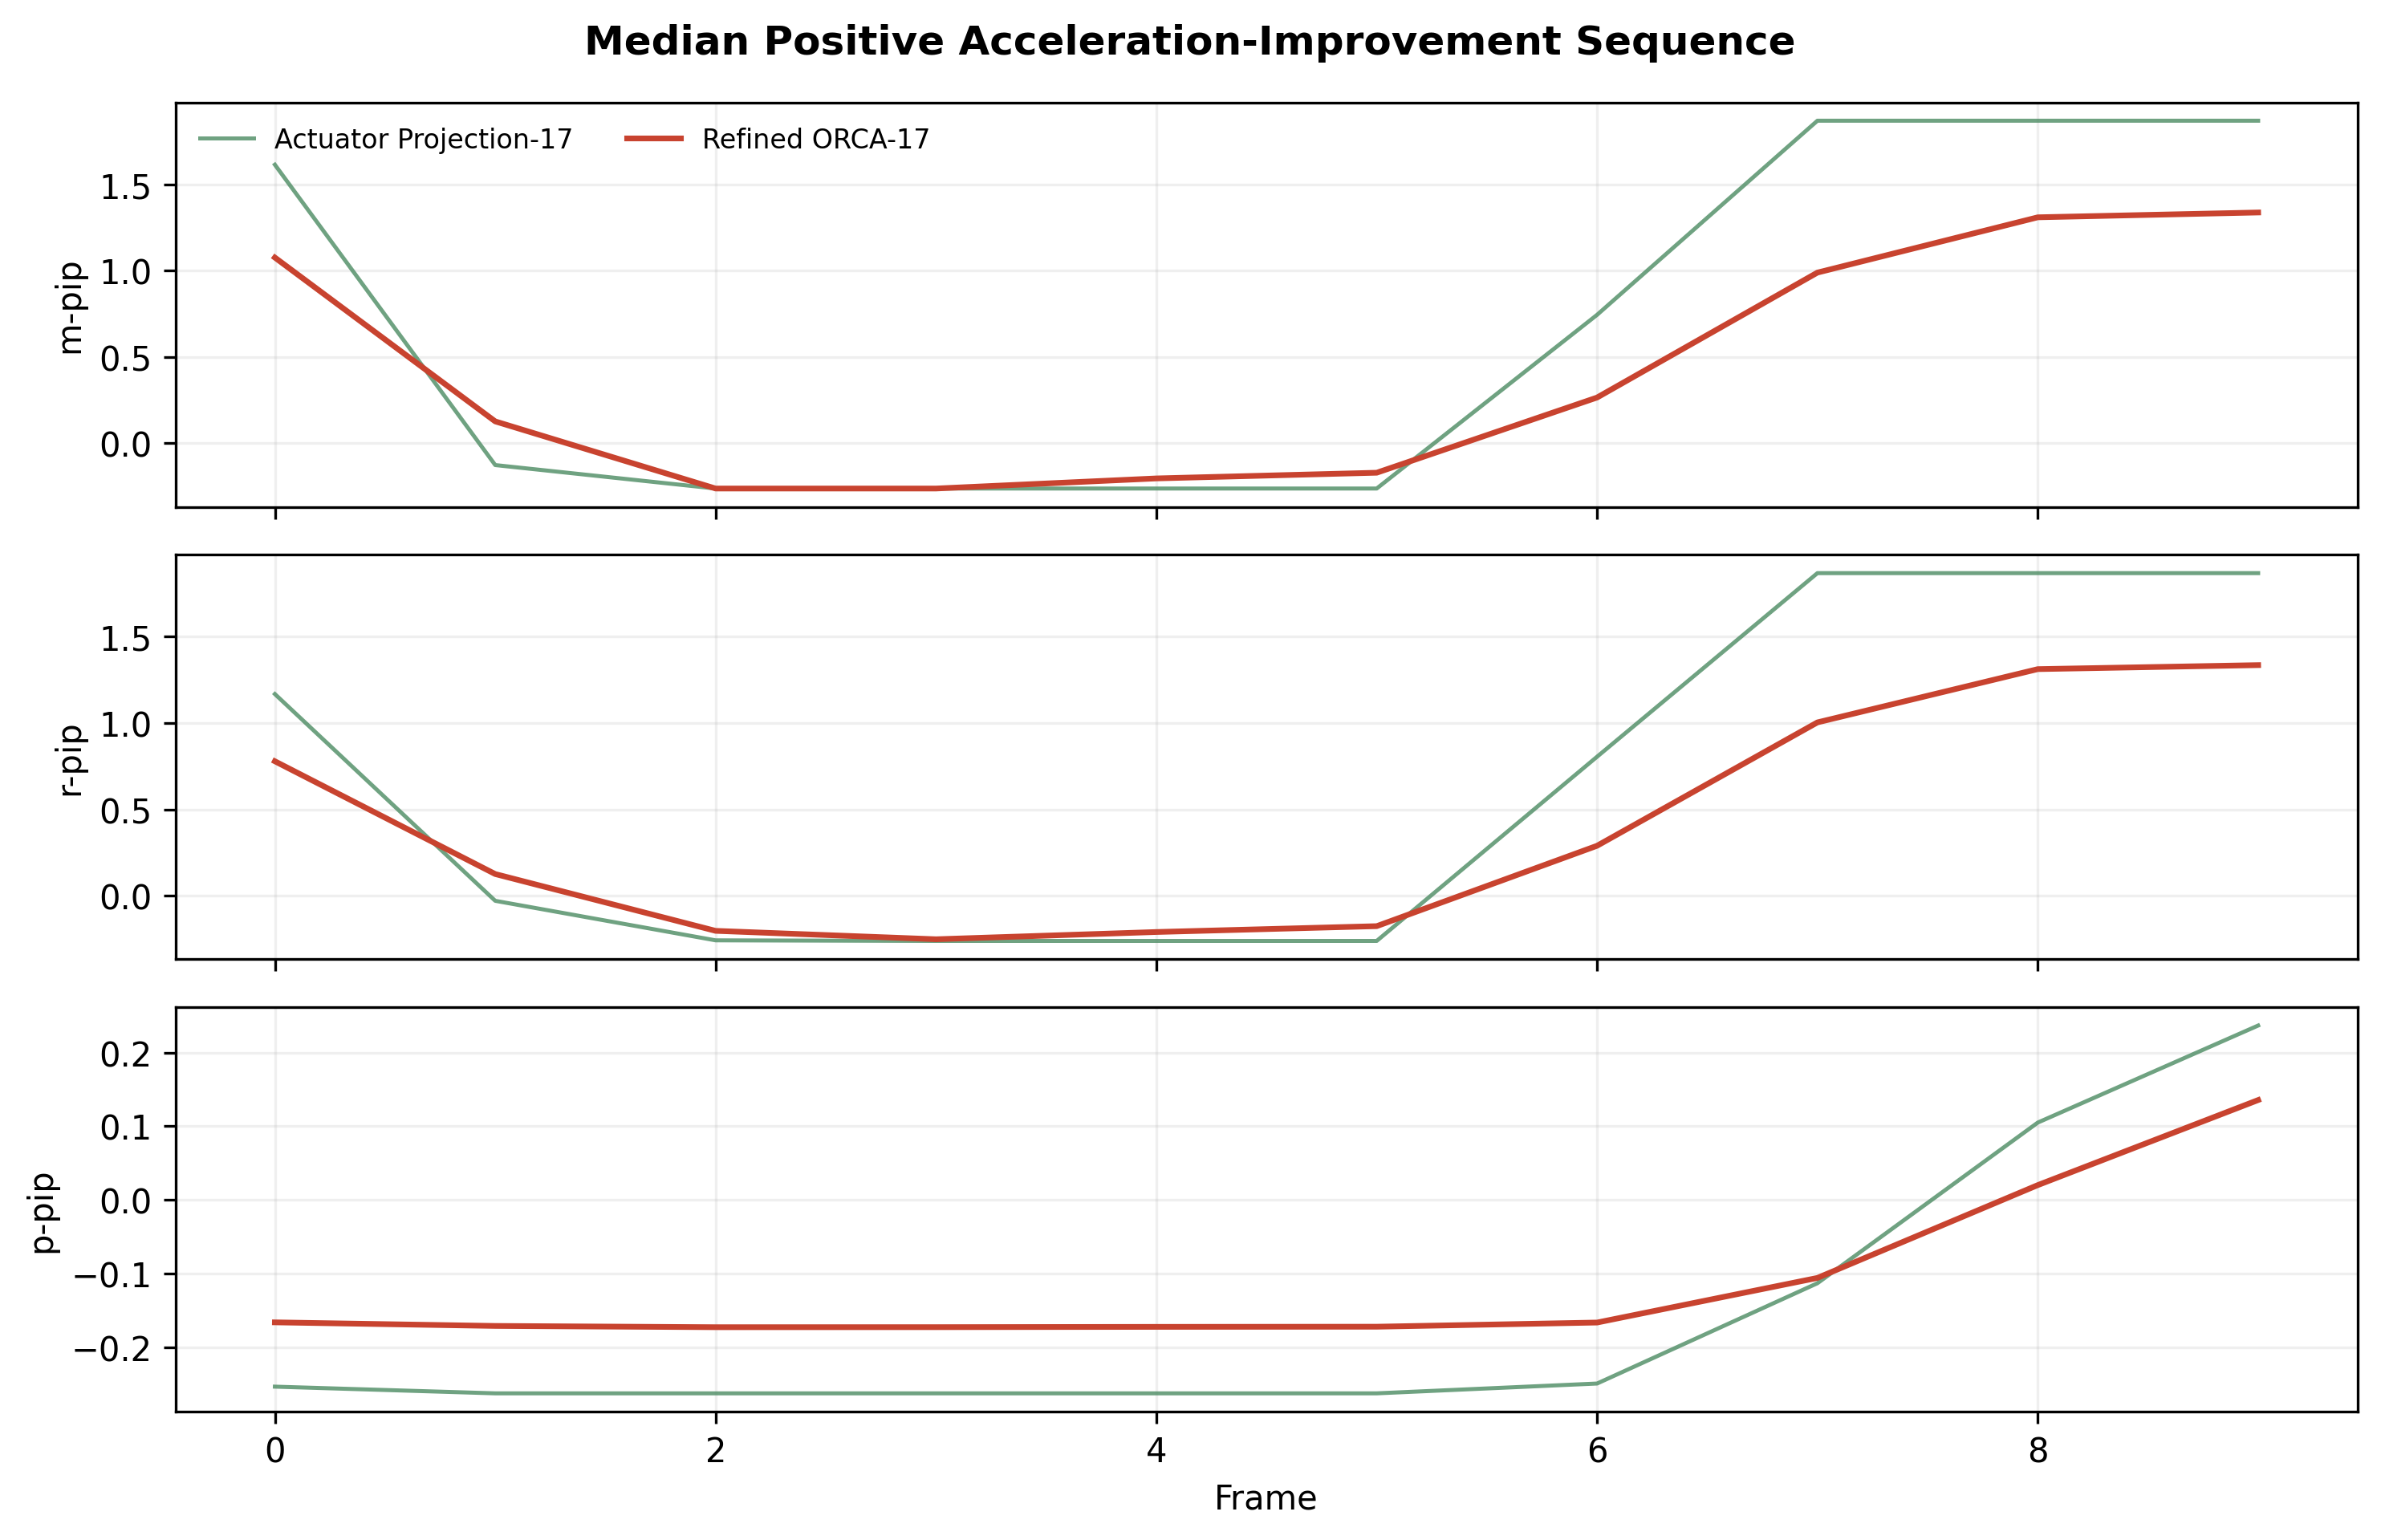
\includegraphics[width=\linewidth]{figure_03_representative_trajectory.png}
\caption{Representative actuator trajectories. The sequence is the median positive sequence-level acceleration improvement, selected systematically from the final stability dataset.}
\label{fig:trajectory}
\end{figure}

\begin{figure}[t]
\centering
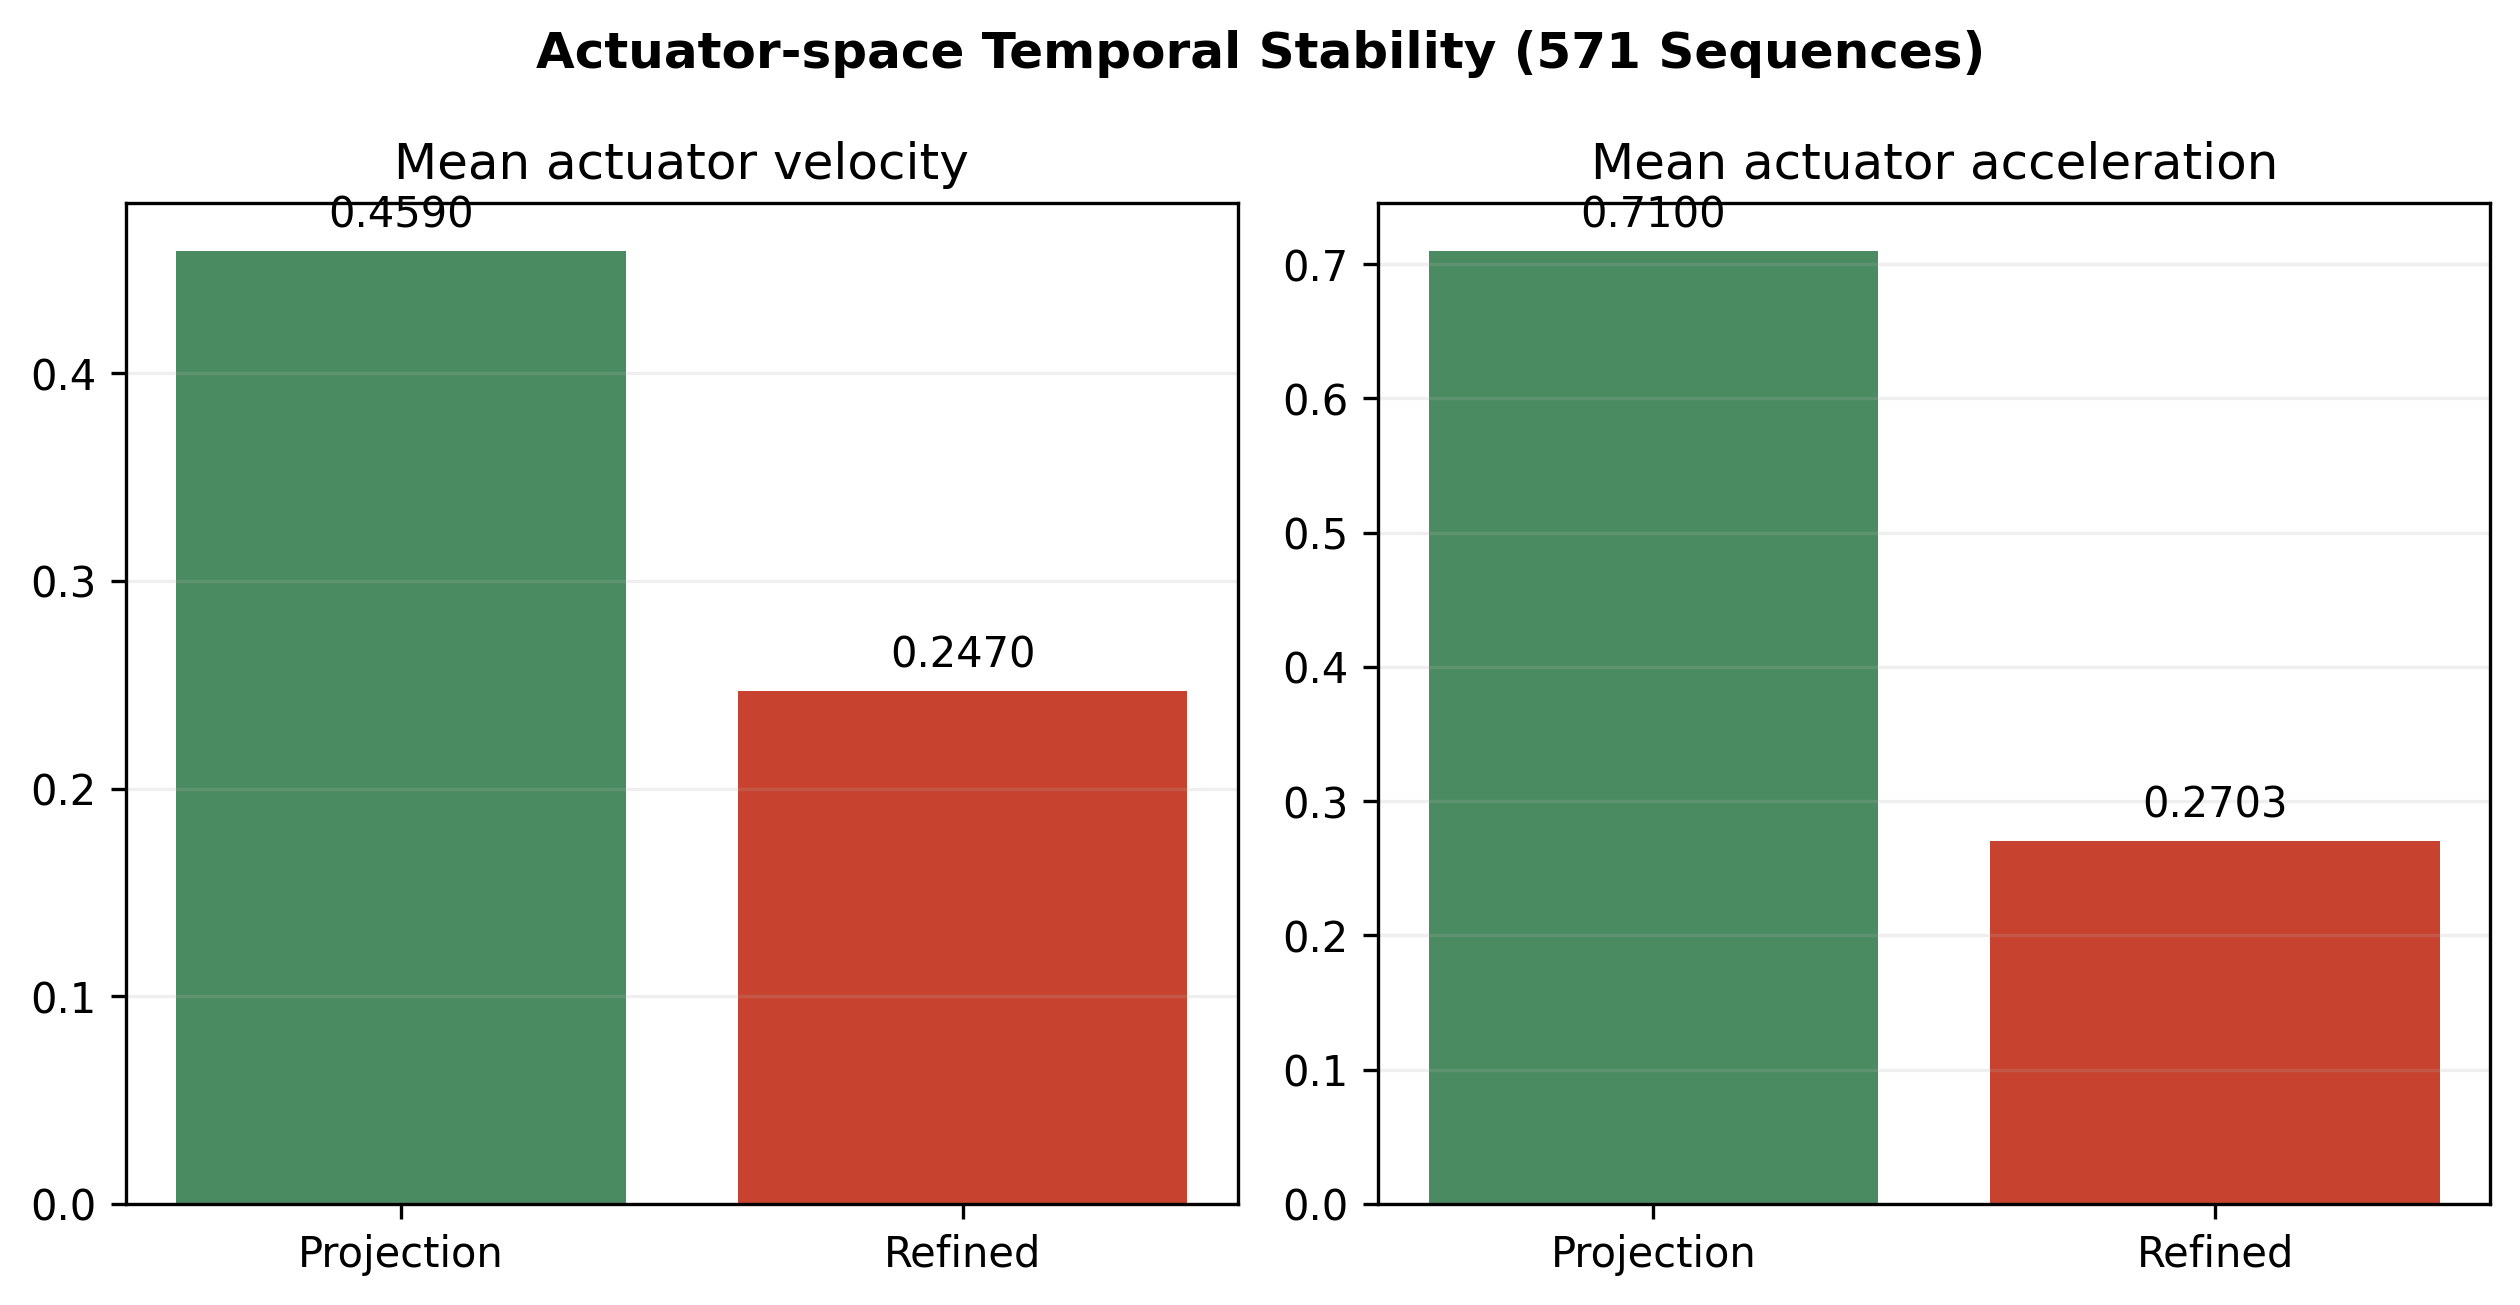
\includegraphics[width=0.85\linewidth]{figure_04_temporal_stability.png}
\caption{Actuator-space temporal stability across 571 sequences. Values from different coordinate spaces are not mixed.}
\label{fig:stability}
\end{figure}

\begin{table}[t]
\centering
\caption{Actuator-space temporal stability.}
\label{tab:stability}
\small
\begin{tabular}{lrrr}
\toprule
Actuator representation & Velocity & Acceleration & Reduction \\
\midrule
Actuator Projection-17 & 0.4590 & 0.7100 & -- \\
Refined ORCA-17 & 0.2470 & 0.2703 & 46.2\% / 61.9\% \\
\bottomrule
\end{tabular}

\end{table}

\subsection{Controlled perturbation sensitivity}
Overall actuator deviation decreases from 0.0292 to 0.0182, a 37.6\% reduction. Reductions are 40.7\% under Gaussian noise, 17.7\% for isolated spikes, and 21.9\% for dropout. These results support robustness of the latent actuator trajectory, not anatomical 3D recovery.

\begin{figure}[t]
\centering
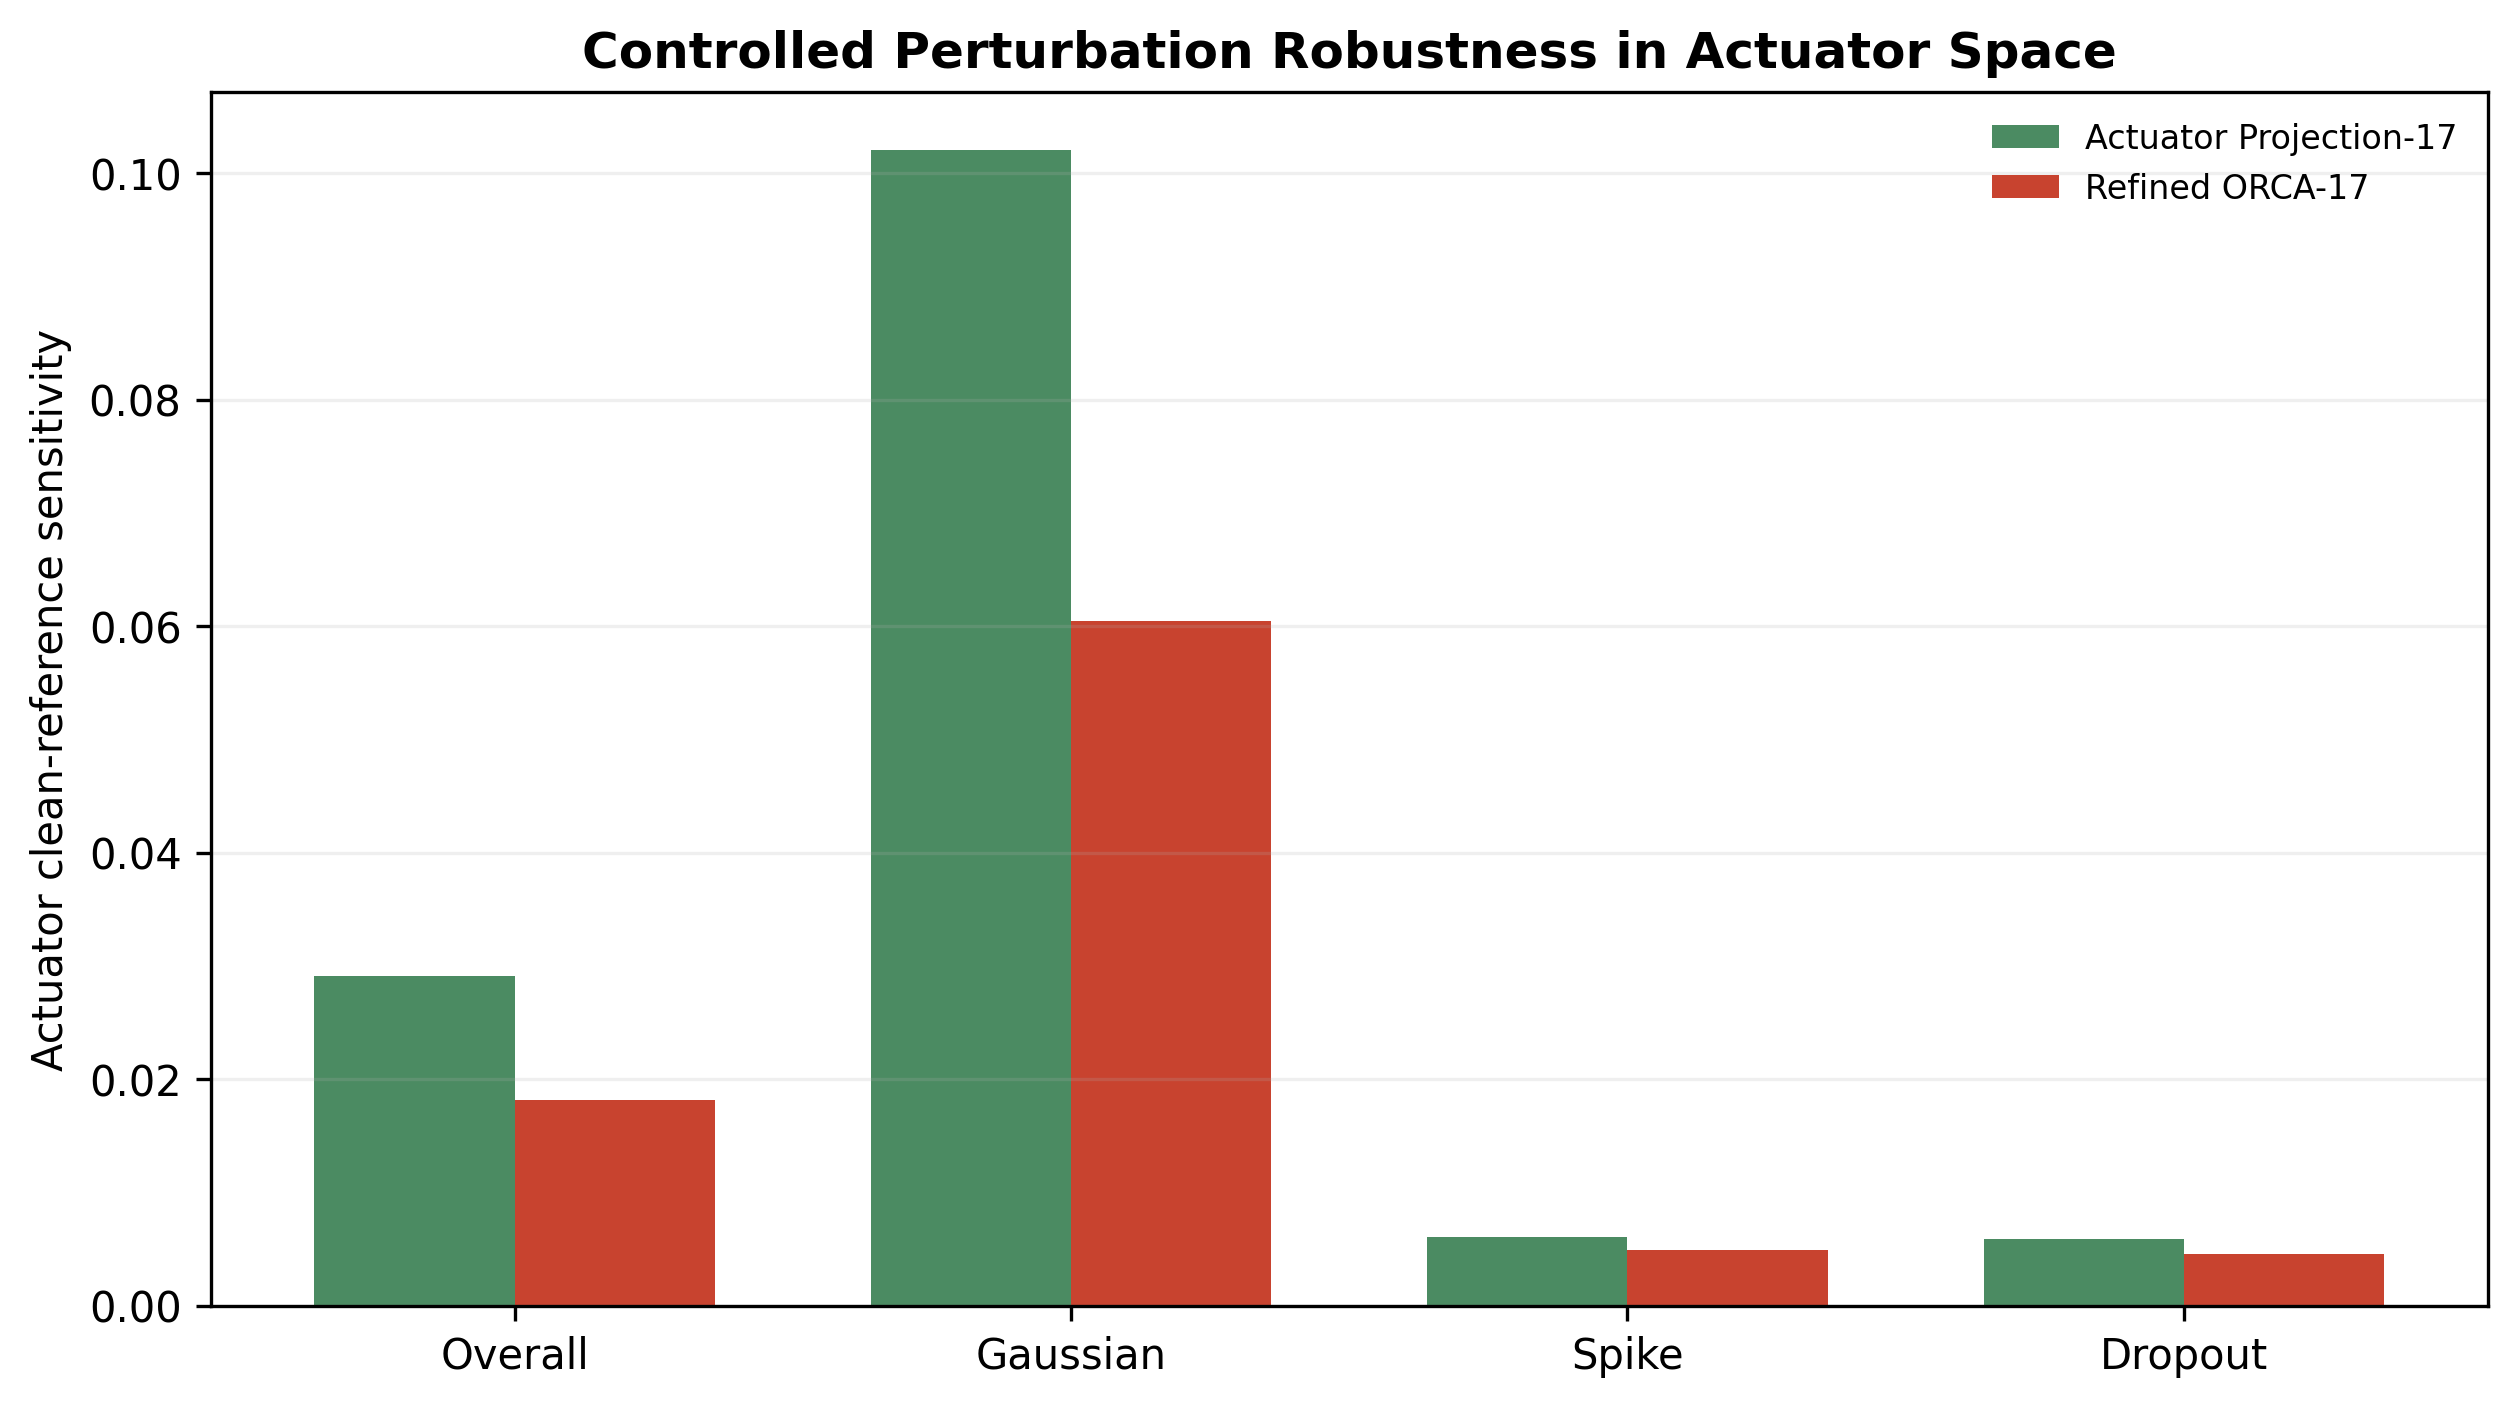
\includegraphics[width=0.78\linewidth]{figure_09_controlled_perturbation.png}
\caption{Actuator sensitivity under controlled input corruption. Lower is better.}
\label{fig:perturbation}
\end{figure}

\begin{table}[t]
\centering
\caption{Controlled perturbation sensitivity.}
\label{tab:perturbation}
\small
\begin{tabular}{lrrr}
\toprule
Condition & Projection-17 & Refined ORCA-17 & Reduction \\
\midrule
Overall & 0.0292 & 0.0182 & 37.6\% \\
Gaussian & 0.1020 & 0.0605 & 40.7\% \\
Spike & 0.0060 & 0.0050 & 17.7\% \\
Dropout & 0.0059 & 0.0046 & 21.9\% \\
\bottomrule
\end{tabular}

\end{table}

\subsection{Development-only compact selection}
The development curve selected $K=7$ before final evaluation (Figure~\ref{fig:development}). Compact Refined-7 uses 112 encoded features, 58.8\% fewer than Refined ORCA-17 and 36.4\% fewer than JointAngle-11.

\begin{figure}[t]
\centering
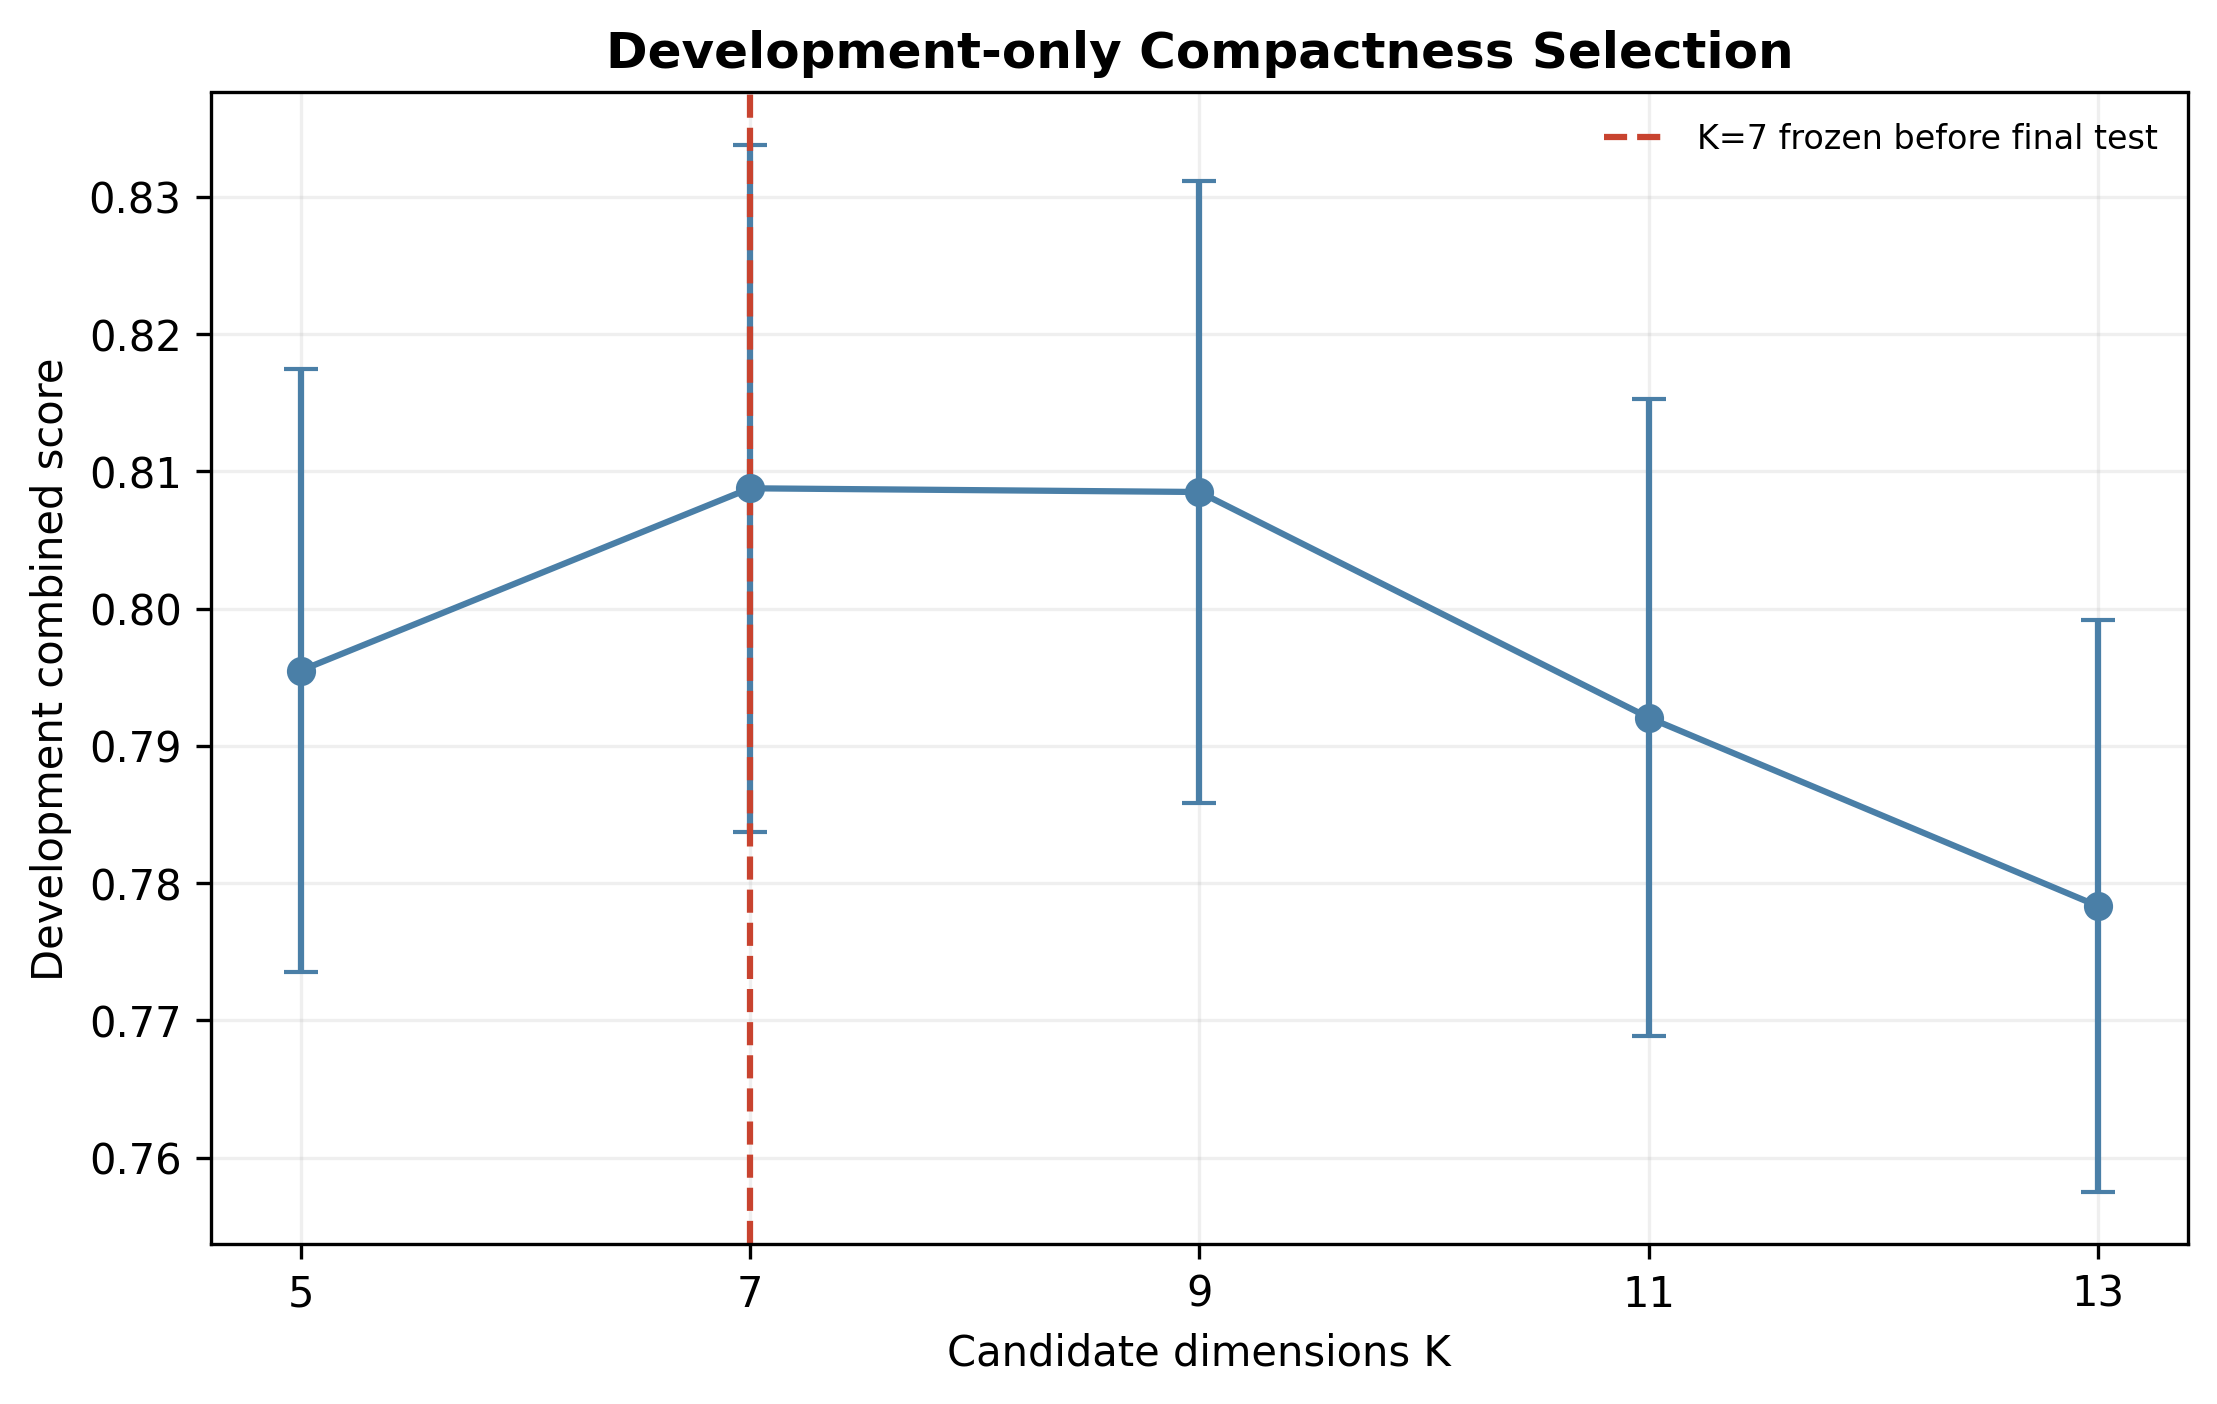
\includegraphics[width=0.72\linewidth]{figure_06_development_selection.png}
\caption{Development-only compactness selection. The final-test labels were not used to select $K$.}
\label{fig:development}
\end{figure}

\subsection{Frozen final classification}
Table~\ref{tab:classification} reports Accuracy/Macro-F1/Kappa. Compact Refined-7 obtains accuracy/macro-F1 of 0.8400/0.8438 with SVM, 0.8070/0.8091 with KNN, 0.8235/0.8222 with RandomForest, and 0.8143/0.8107 with MLP.

Compared with JointAngle-11, repeat-wise accuracy differences are $+0.0374$ for SVM, $+0.0448$ for KNN, $-0.0087$ for RandomForest, and $+0.0183$ for MLP. After Holm correction, SVM and KNN improvements are significant; RandomForest and MLP differences are not. Compact Refined-7 also improves over Refined ORCA-17 for SVM, KNN, and MLP, while RandomForest is approximately unchanged.

\begin{table}[t]
\centering
\caption{Frozen final classification. Each entry is Accuracy / Macro-F1 / Kappa.}
\label{tab:classification}
\scriptsize
\resizebox{\linewidth}{!}{\begin{tabular}{lrrrr}
\toprule
Representation & SVM & KNN & RF & MLP \\
\midrule
JointAngle-11 & 0.8026 / 0.8082 / 0.7629 & 0.7622 / 0.7605 / 0.7142 & 0.8322 / 0.8331 / 0.7985 & 0.7961 / 0.7972 / 0.7549 \\
Actuator Projection-17 & 0.7883 / 0.7946 / 0.7460 & 0.7552 / 0.7453 / 0.7063 & 0.8330 / 0.8317 / 0.7996 & 0.7961 / 0.7939 / 0.7553 \\
Refined ORCA-17 & 0.8013 / 0.8068 / 0.7615 & 0.7457 / 0.7336 / 0.6947 & 0.8252 / 0.8249 / 0.7902 & 0.7748 / 0.7721 / 0.7298 \\
Projection Flex-11 & 0.8096 / 0.8154 / 0.7714 & 0.7800 / 0.7805 / 0.7357 & 0.8348 / 0.8359 / 0.8017 & 0.8122 / 0.8106 / 0.7744 \\
Refined Flex-11 & 0.8117 / 0.8177 / 0.7740 & 0.7765 / 0.7766 / 0.7315 & 0.8209 / 0.8215 / 0.7850 & 0.8165 / 0.8168 / 0.7796 \\
Compact Projection-7 & 0.8339 / 0.8382 / 0.8004 & 0.8039 / 0.8066 / 0.7642 & 0.8339 / 0.8335 / 0.8006 & 0.8061 / 0.8026 / 0.7668 \\
Compact Refined-7 & 0.8400 / 0.8438 / 0.8077 & 0.8070 / 0.8091 / 0.7678 & 0.8235 / 0.8222 / 0.7881 & 0.8143 / 0.8107 / 0.7768 \\
\bottomrule
\end{tabular}
}
\end{table}

\begin{figure}[t]
\centering
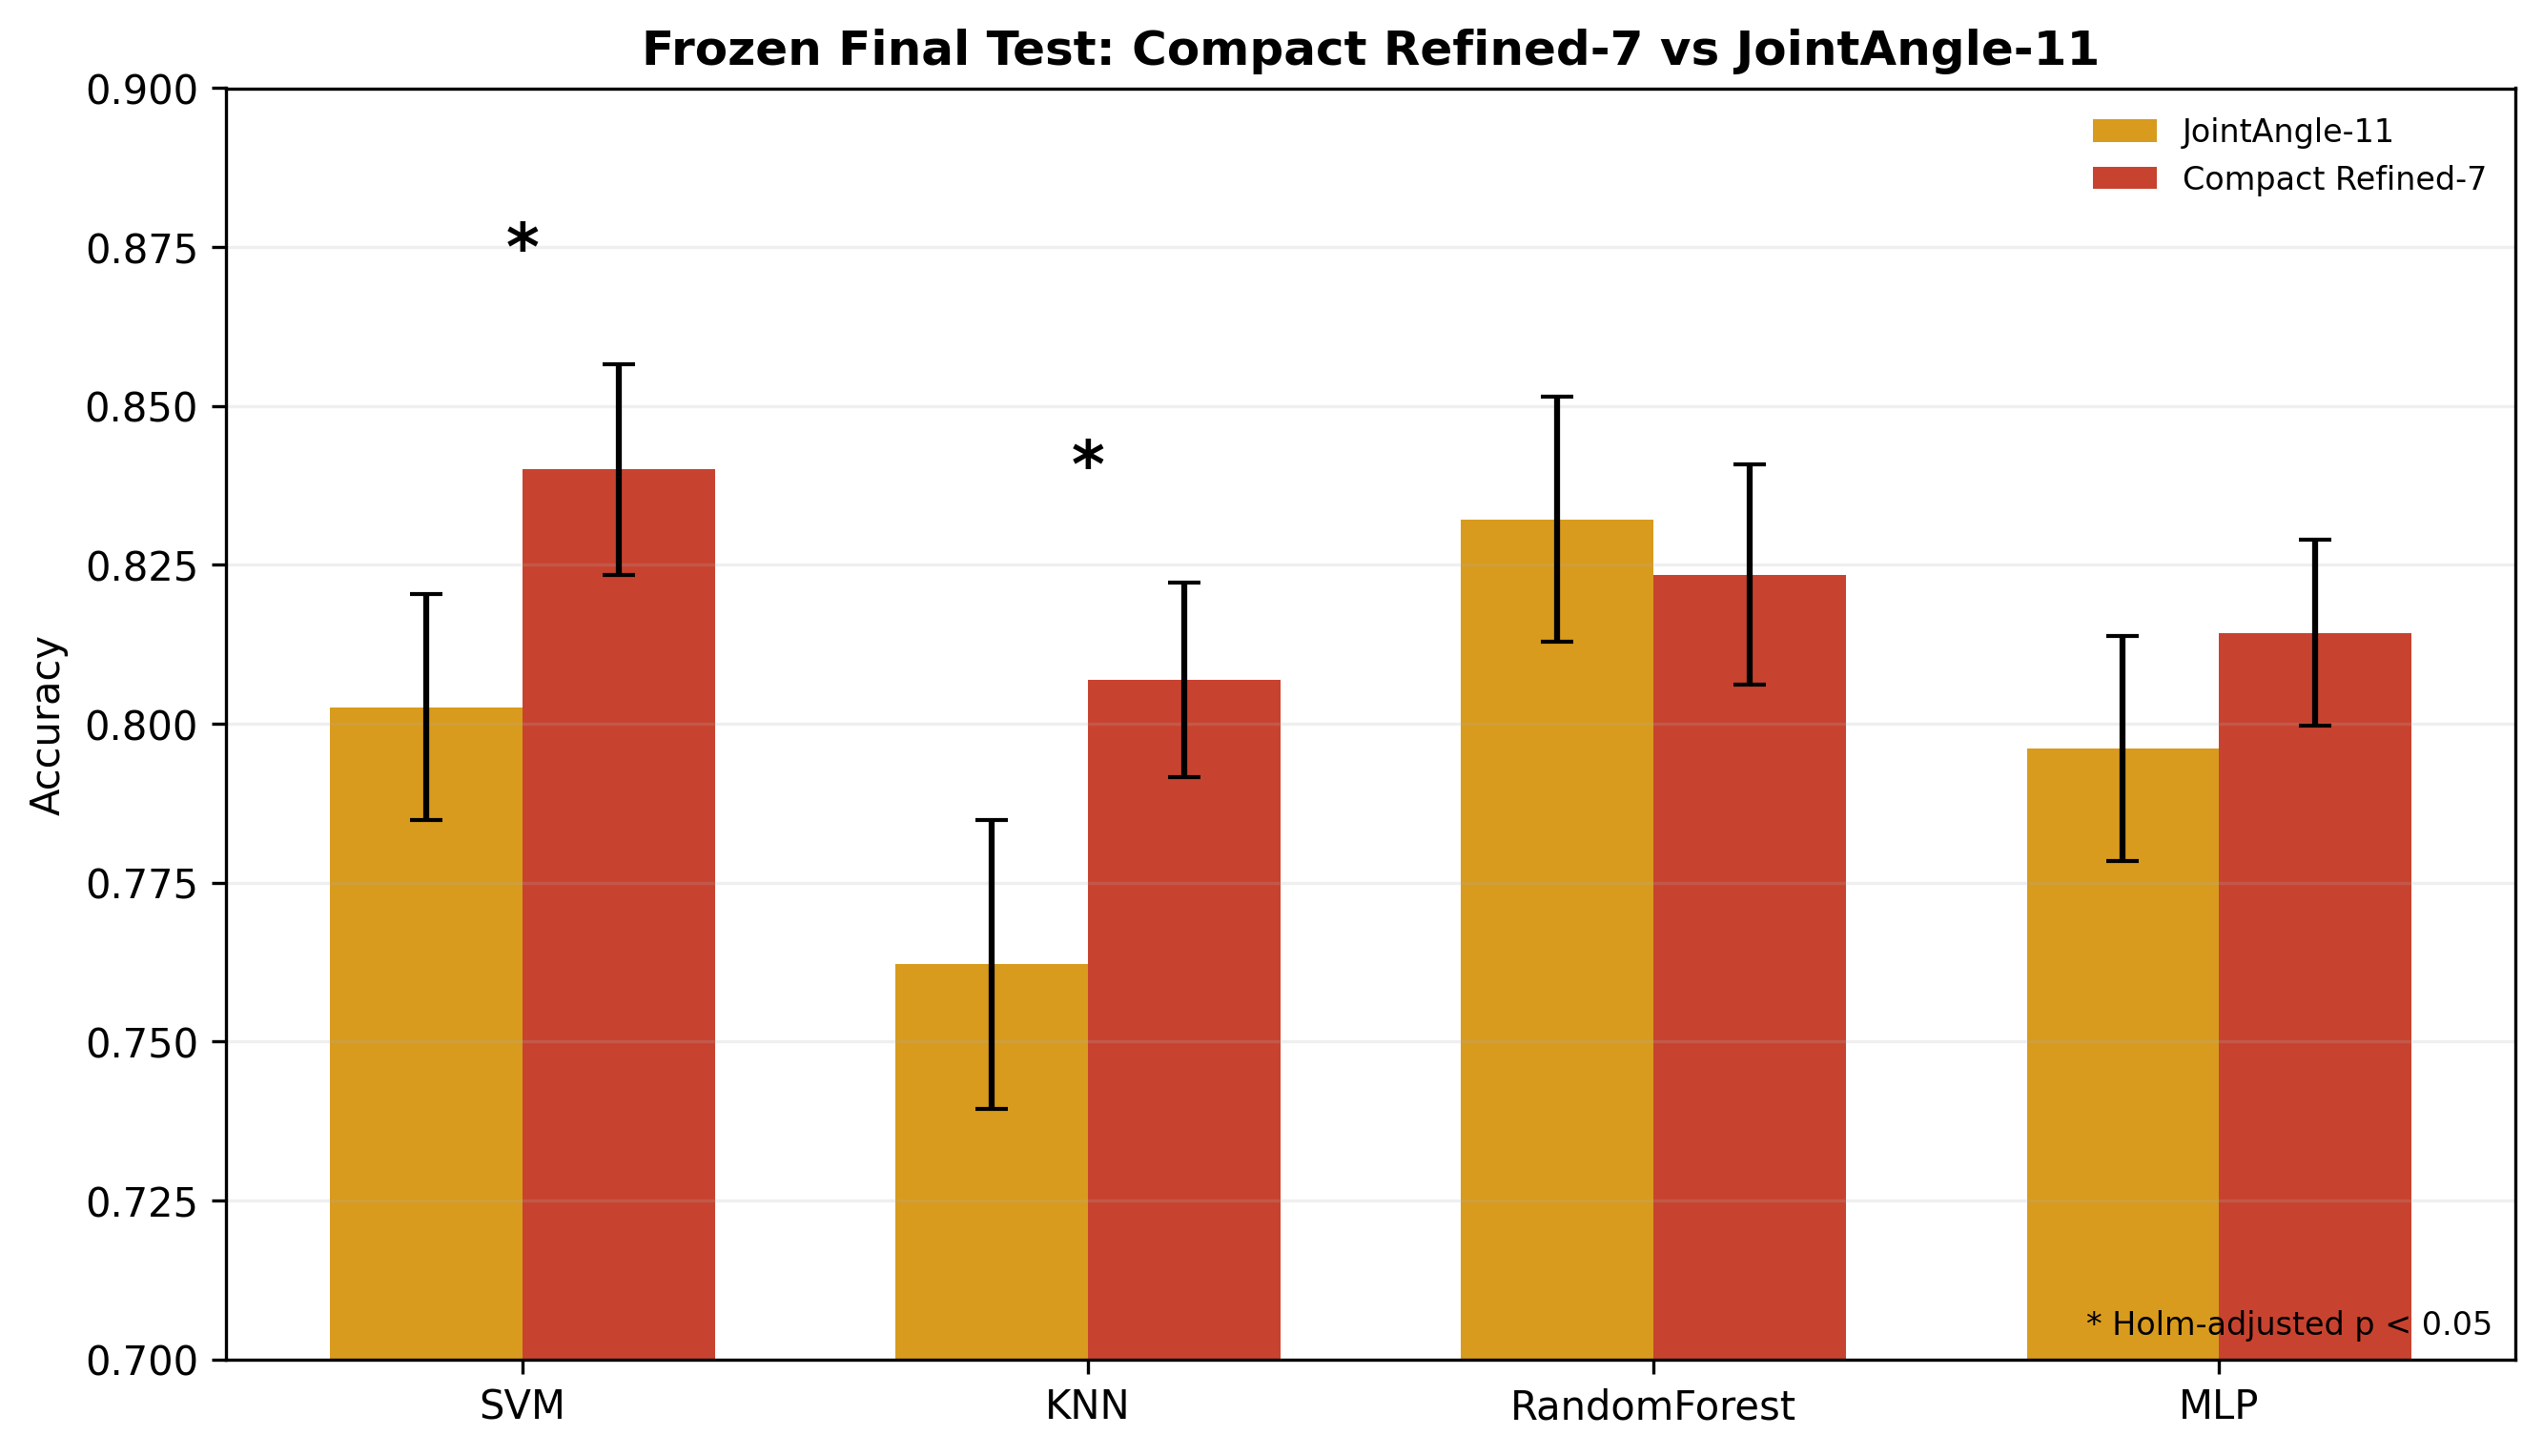
\includegraphics[width=0.9\linewidth]{figure_07_final_compact_vs_jointangle.png}
\caption{Frozen final-test accuracy. Stars denote Holm-adjusted $p<0.05$ for the Compact Refined-7 versus JointAngle-11 paired comparison.}
\label{fig:final}
\end{figure}

\begin{table}[t]
\centering
\caption{Paired Compact Refined-7 minus JointAngle-11 comparisons. Confidence intervals are mean difference $\pm$ the reported 95\% half-width.}
\label{tab:paired}
\scriptsize
\resizebox{\linewidth}{!}{\begin{tabular}{lllrrr}
\toprule
Classifier & Metric & Difference & 95\% CI & Holm p & dz \\
\midrule
SVM & accuracy & +0.0374 & [+0.0182, +0.0566] & 0.01106 & +0.854 \\
SVM & macro\_f1 & +0.0356 & [+0.0171, +0.0541] & 0.004253 & +0.844 \\
KNN & accuracy & +0.0448 & [+0.0277, +0.0618] & 0.002125 & +1.151 \\
KNN & macro\_f1 & +0.0486 & [+0.0281, +0.0691] & 0.0006714 & +1.038 \\
RandomForest & accuracy & -0.0087 & [-0.0282, +0.0108] & 1 & -0.195 \\
RandomForest & macro\_f1 & -0.0109 & [-0.0312, +0.0095] & 1 & -0.234 \\
MLP & accuracy & +0.0183 & [+0.0014, +0.0351] & 0.1397 & +0.475 \\
MLP & macro\_f1 & +0.0135 & [-0.0036, +0.0306] & 0.7574 & +0.345 \\
\bottomrule
\end{tabular}
}
\end{table}

\begin{figure}[t]
\centering
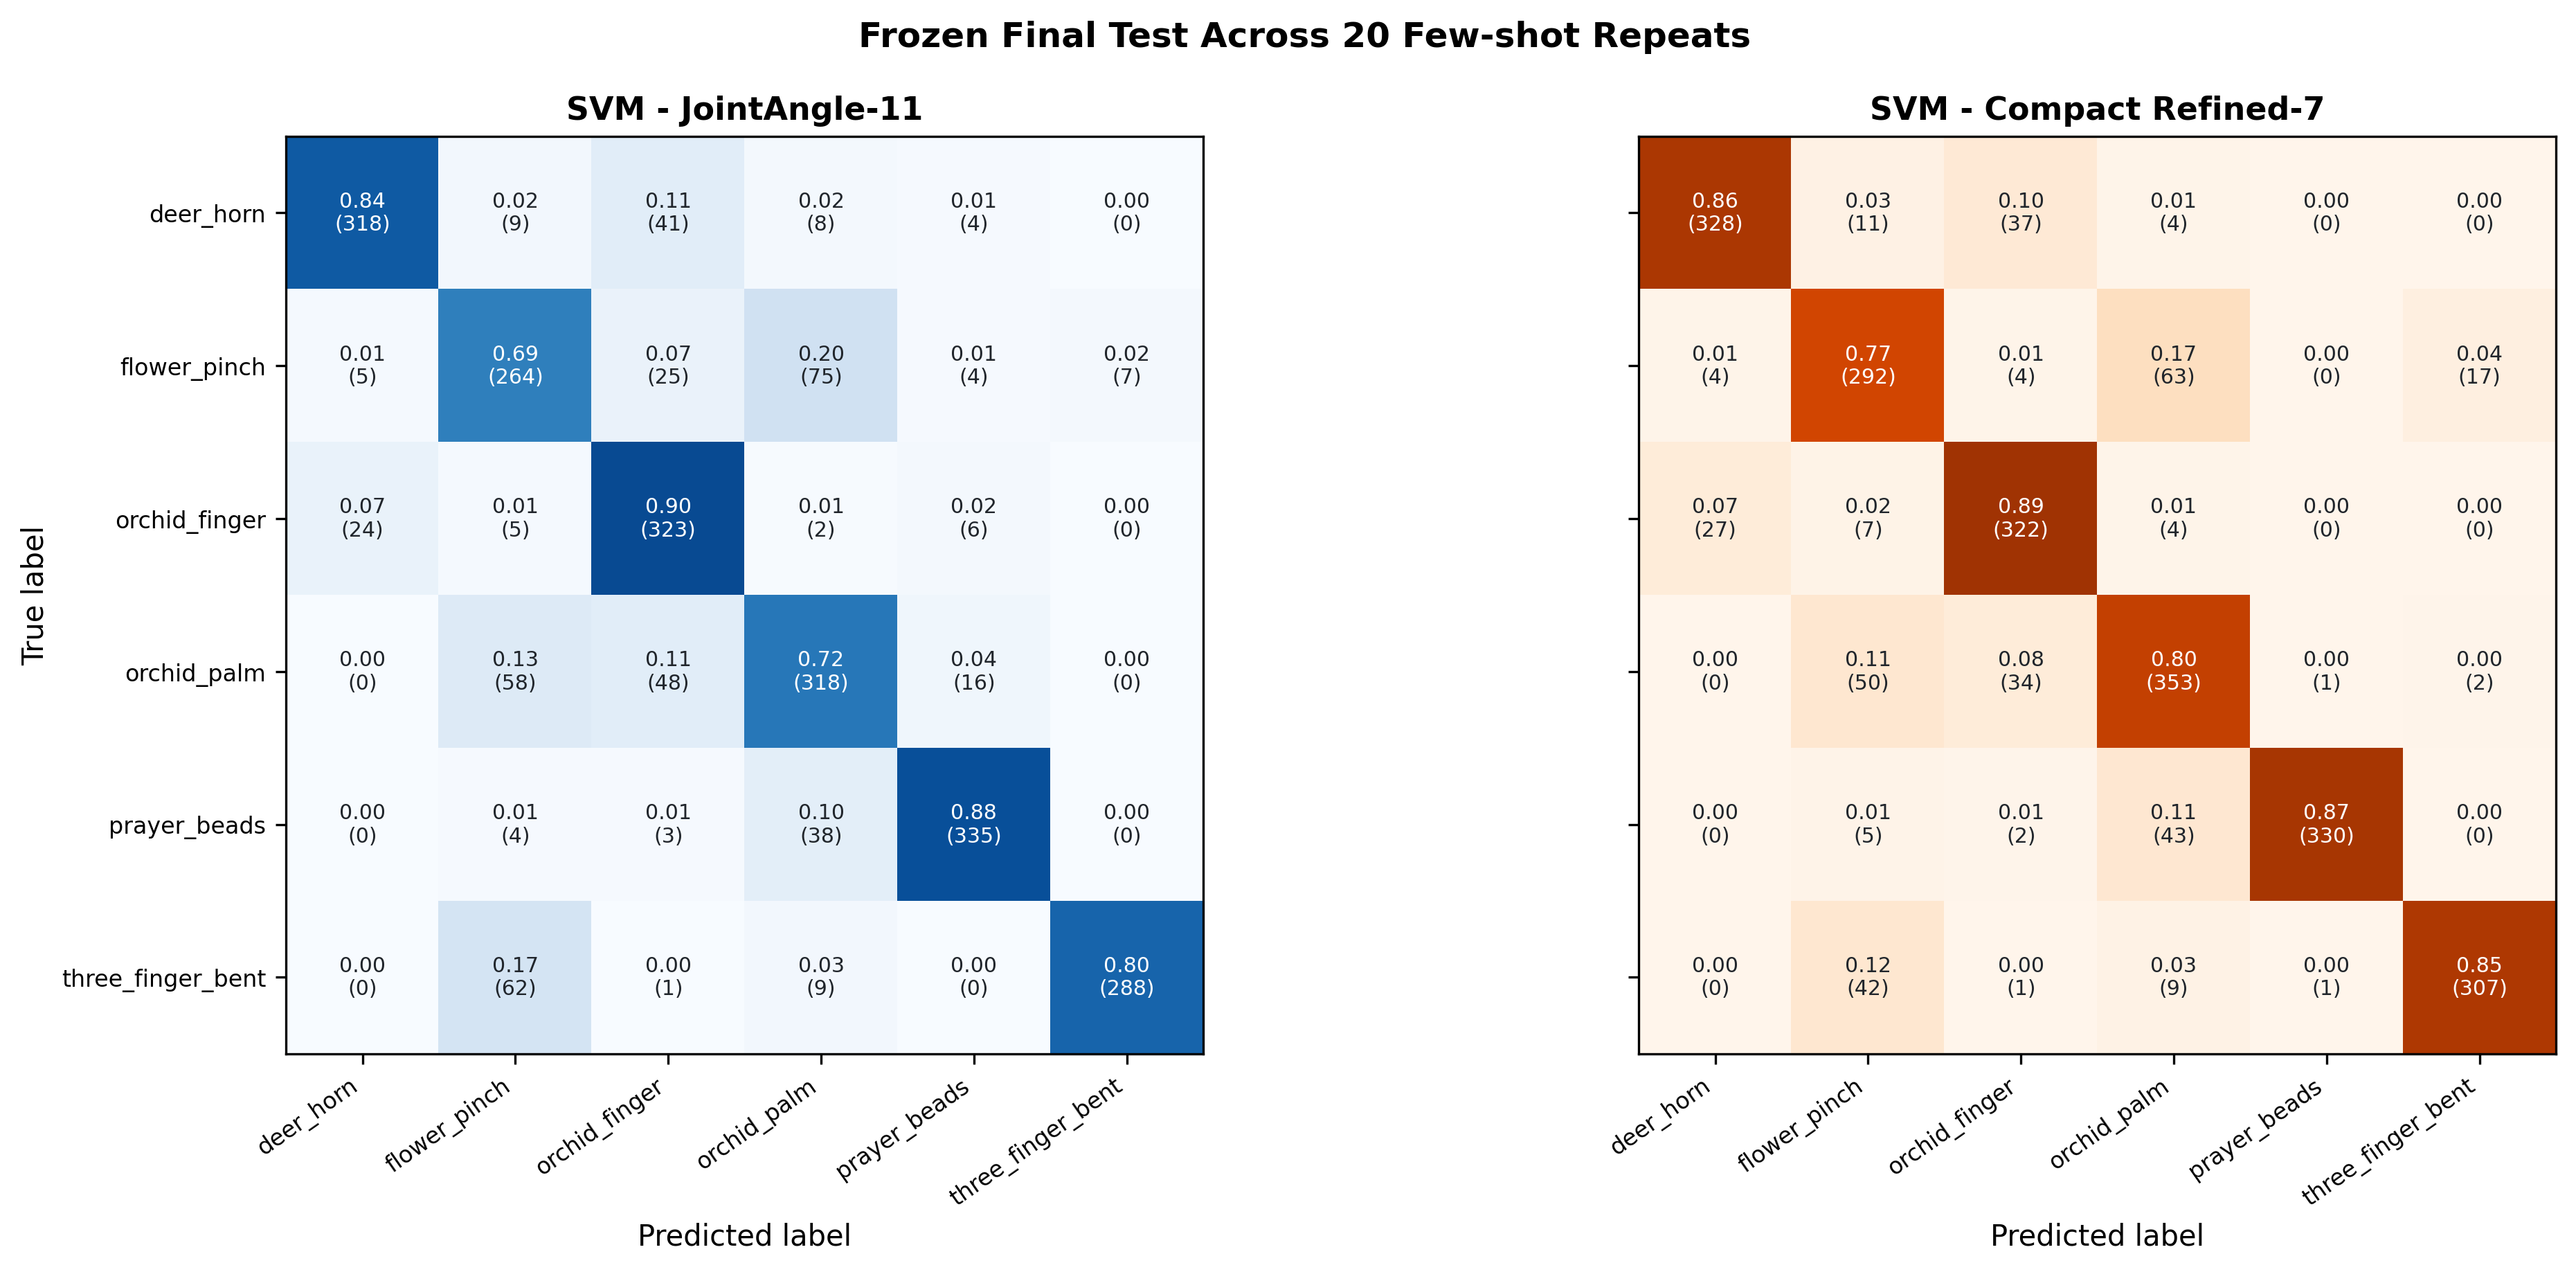
\includegraphics[width=\linewidth]{figure_10_main_svm_confusion_comparison.png}
\caption{Aggregate SVM confusion matrices for JointAngle-11 and Compact Refined-7 across the 20 frozen few-shot repeats. Each cell shows row-normalized frequency and cumulative count. Because the same 115 final sequences are evaluated repeatedly, cumulative counts are descriptive repeated predictions rather than independent test samples.}
\label{fig:confusion}
\end{figure}

Per-cell means and sample standard deviations of the 20 repeat-level row-normalized confusion matrices are provided in the supplementary workbook and figures. They quantify sensitivity to few-shot training selection and are distinct from actuator-space temporal stability.

\subsection{Dimension-controlled evidence}
Flexion-only and PCA-controlled representations show that dimensionality alone does not explain performance. Compact Refined-7 combines low dimension with explicit semantic coverage and a frozen selection rule; we do not claim universal superiority over PCA.

This dimension-controlled evidence answers RQ1: the actuator projection is competitive as a bounded semantic representation, but it is not claimed to dominate every statistical or geometric representation for every classifier.

\begin{figure}[t]
\centering
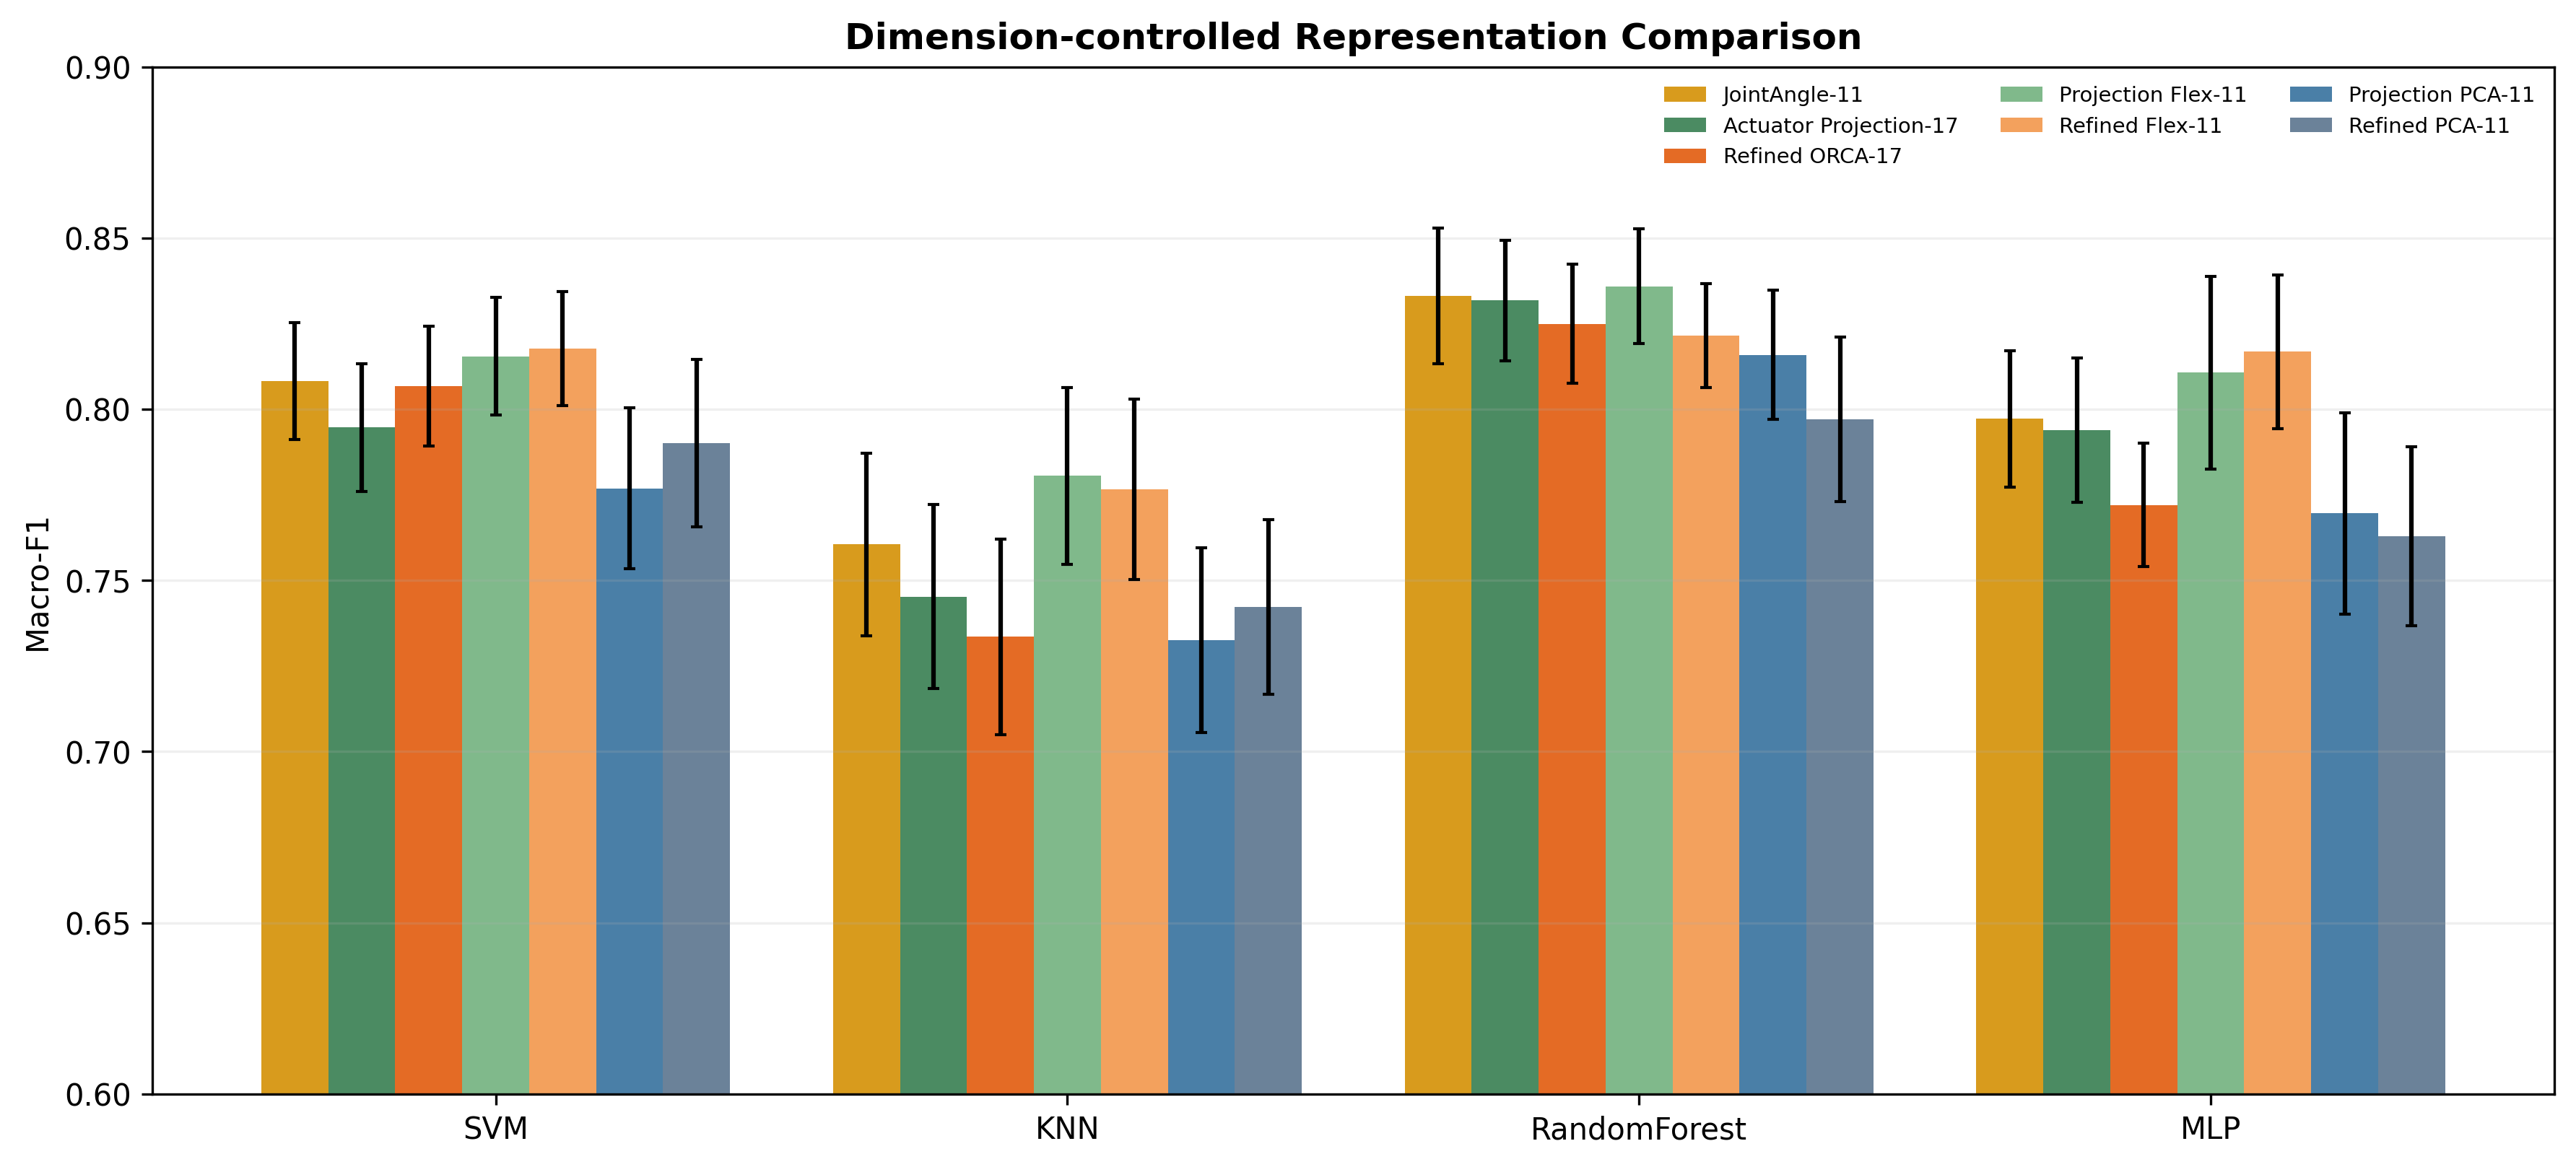
\includegraphics[width=\linewidth]{figure_05_dimension_control.png}
\caption{Dimension-controlled Macro-F1 comparison on the frozen final test.}
\label{fig:dimensioncontrol}
\end{figure}

\begin{figure}[t]
\centering
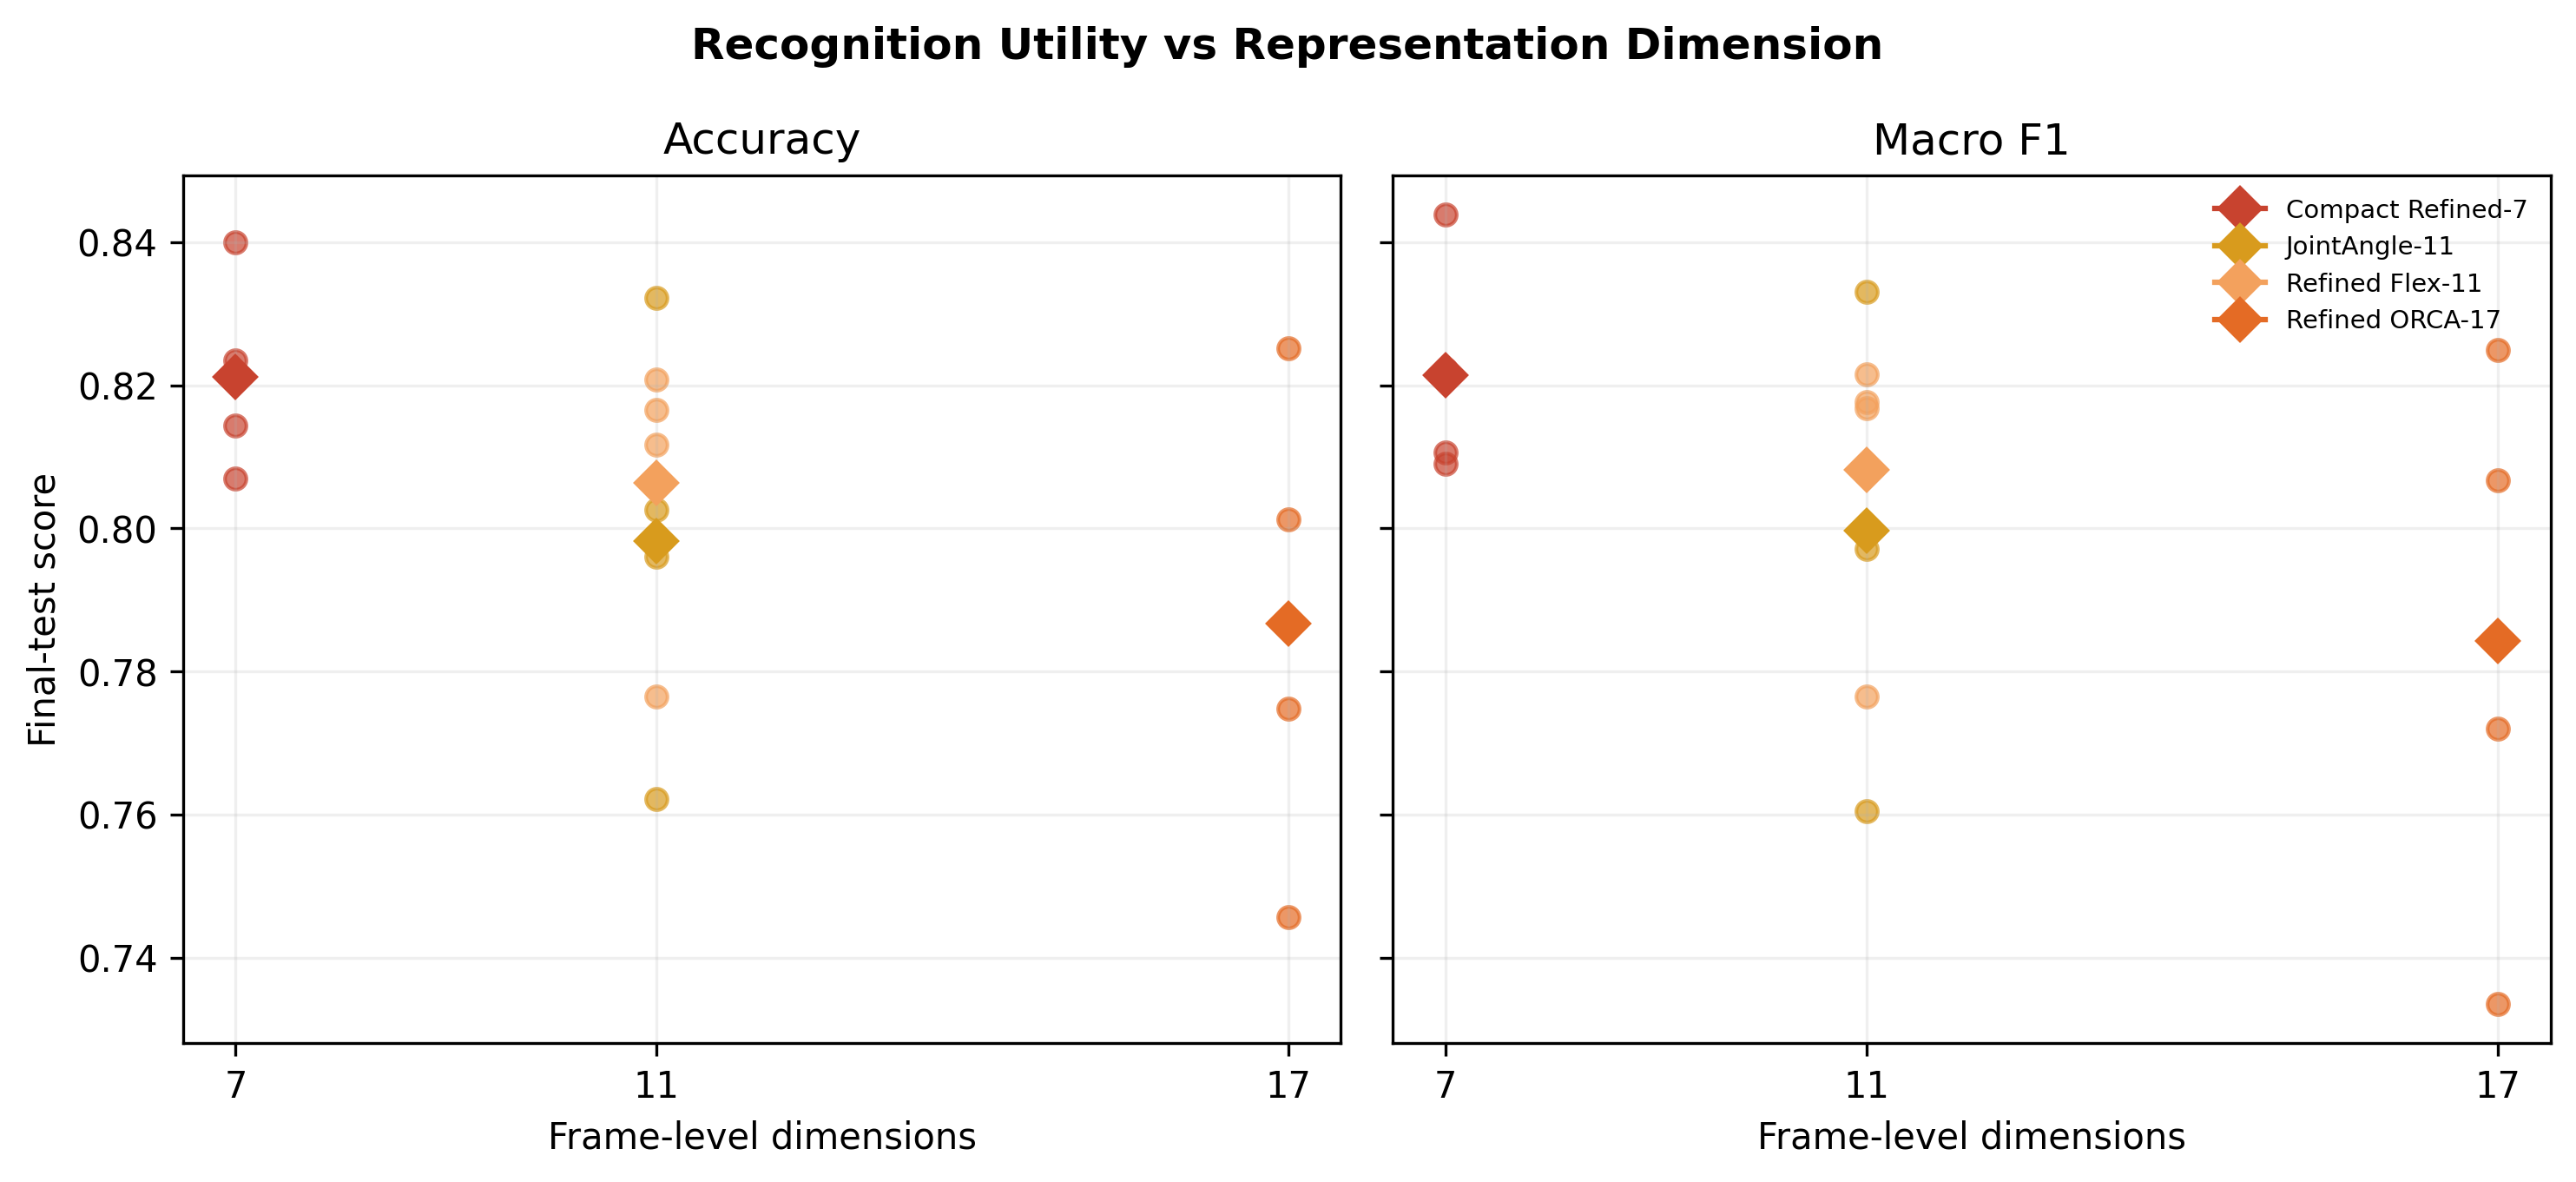
\includegraphics[width=0.85\linewidth]{figure_08_performance_vs_dimension.png}
\caption{Recognition accuracy versus frame-level representation dimension.}
\label{fig:dimension}
\end{figure}

\subsection{Ablation and runtime}
Removing temporal terms increases actuator velocity and acceleration. L2 fitting reduces supporting classification performance relative to Huber fitting. Palm-normal removal has a smaller effect and is not overstated. Runtime averages 27.61 ms per frame (median 27.27 ms; 95th percentile 32.62 ms), with 6.02 mean iterations and 100\% successful finite outputs. This supports \emph{causal frame-wise refinement}, not a hardware-independent real-time claim.

\begin{table}[t]
\centering
\caption{Supporting objective ablation. Classification values are supporting results, not the frozen Compact Refined-7 final comparison.}
\label{tab:ablation}
\small
\begin{tabular}{lrrrr}
\toprule
Variant & Velocity & Acceleration & SVM Acc. & RF Acc. \\
\midrule
corrected & 0.4590 & 0.7100 & 0.7491 & 0.7826 \\
full & 0.2470 & 0.2703 & 0.7278 & 0.7674 \\
no\_palm & 0.2391 & 0.2646 & 0.7378 & 0.7717 \\
no\_acceleration & 0.2685 & 0.3718 & 0.7213 & 0.7730 \\
no\_temporal & 0.3238 & 0.4976 & 0.7096 & 0.7609 \\
l2 & 0.2560 & 0.2926 & 0.6548 & 0.7335 \\
\bottomrule
\end{tabular}

\end{table}

\begin{table}[t]
\centering
\caption{Runtime and convergence diagnostics.}
\label{tab:runtime}
\small
\resizebox{\linewidth}{!}{\begin{tabular}{rrrrrr}
\toprule
Frames & Mean ms & Median ms & P95 ms & Iterations & Success \\
\midrule
300 & 27.61 & 27.27 & 32.62 & 6.02 & 100\% \\
\bottomrule
\end{tabular}
}
\end{table}

\FloatBarrier
\section{Discussion}

\subsection{Distinct roles of projection, refinement, and compact readout}
The frame-wise projection is a strong discriminative representation because it converts raw coordinates into bounded articulation variables. The optimizer need not beat that initialization for every classifier to be meaningful: its demonstrated role is temporal stability and perturbation robustness. Compact selection removes channels that are less useful under the target recognition protocol.

This interpretation resolves earlier results in which Actuator Projection-17 sometimes classified better than Refined ORCA-17. Classification and smoothness are different objectives. Temporal regularization can suppress informative amplitude as well as noise, and 17 actuator channels can contain redundancy. Compact Refined-7 gives a better trade-off without changing the frozen optimizer.

\subsection{Not ordinary coordinate smoothing}
Coordinate filters can be stronger direct landmark smoothers. The proposed method instead searches a bounded actuator state whose points are generated by an articulated MuJoCo model. Its contribution is a structured latent trajectory, not a claim that MuJoCo always produces the smoothest coordinates. Reconstructed ORCA Landmarks may show clean-domain reconstruction bias because ORCA geometry is not ground-truth human anatomy.

\subsection{Classifier-dependent evidence}
SVM and KNN benefit most from Compact Refined-7, suggesting useful margins and neighborhoods in the compact actuator geometry. RandomForest slightly favors JointAngle-11 in mean accuracy, without a significant paired difference. MLP shows a positive but non-significant difference. Reporting these outcomes together avoids cherry-picking a favorable classifier.

\section{Limitations}
\begin{enumerate}[leftmargin=*]
\item The current dataset does not establish subject-independent generalization; multi-participant and multi-session validation is needed.
\item There is no synchronized ground-truth 3D human hand pose. Stability and controlled corruption sensitivity are not anatomical reconstruction accuracy.
\item ORCA is a robotic embodiment and does not exactly match human joint axes or bone lengths.
\item The current right-hand acquisition convention is not general left/right canonicalization.
\item Compact Refined-7 requires external validation before being treated as universal.
\item JointAngle-11 follows a published geometric definition but is not a full reproduction of the source system.
\item Resample16 preserves coarse order but is not a learned long-range temporal model.
\item Synthetic corruption approximates observation failures and cannot reproduce every real occlusion pattern.
\end{enumerate}

\section{Conclusion}
This study presents a compact ORCA actuator representation with MuJoCo-constrained causal temporal refinement for few-shot Chinese dance gesture recognition. The evidence supports three specific conclusions. First, ORCA actuator projection provides an interpretable structured representation of MediaPipe landmarks. Second, causal MuJoCo refinement substantially reduces actuator-space temporal variation and sensitivity to controlled landmark corruption. Third, a seven-actuator subset frozen using development data reduces encoded dimensionality and improves frozen final-test performance over JointAngle-11 for SVM and KNN, while RandomForest and MLP differences are not significant after correction. The method should therefore be understood as a compact, model-consistent representation and refinement framework, not as ground-truth 3D hand recovery or a universally superior classifier input.

\section*{Author Contributions}
\textbf{[TODO: insert a CRediT-style statement identifying conceptualization, software, data collection, analysis, visualization, supervision, and writing.]}

\section*{Institutional Review Board Statement}
\textbf{[TODO: insert the approving institution and identifier, or the accurate exemption/waiver statement.]}

\section*{Informed Consent Statement}
\textbf{[TODO: state how participant consent and permission to publish identifiable images or video were obtained.]}

\section*{Data Availability Statement}
\textbf{[TODO: insert repository information, a controlled-access procedure, or a justified restriction.]}

\section*{Funding}
\textbf{[TODO: insert funder and grant number, or state that the research received no external funding.]}

\section*{Conflicts of Interest}
\textbf{[TODO: insert the authors' declaration.]}

\bibliographystyle{plain}
\bibliography{references}
\end{document}
